

%----------------------------------------------------------------------------------------
%	PACKAGES AND OTHER DOCUMENT CONFIGURATIONS
%----------------------------------------------------------------------------------------

\documentclass[11pt, a4paper, oneside]{Thesis} % Paper size, default font size and one-sided paper

\graphicspath{{./Pictures/}} % Specifies the directory where pictures are stored

\usepackage[square, numbers, comma, sort&compress]{natbib}
\usepackage{subfigure}
\usepackage{caption}
\usepackage{graphicx}
\usepackage{import}
\usepackage{pdfpages}
%\usepackage{showframe}  


%\usepackage{subcaption}
 % Use the natbib reference package - read up on this to edit the reference style; if you want text (e.g. Smith et al., 2012) for the in-text references (instead of numbers), remove 'numbers' 
\hypersetup{urlcolor=blue, colorlinks=true} % Colors hyperlinks in blue - change to black if annoying
\title{\ttitle} % Defines the thesis title - don't touch this



\begin{document}

\frontmatter % Use roman page numbering style (i, ii, iii, iv...) for the pre-content pages

\setstretch{1.3} % Line spacing of 1.3

% Define the page headers using the FancyHdr package and set up for one-sided printing
\fancyhead{} % Clears all page headers and footers
\rhead{\thepage} % Sets the right side header to show the page number
\lhead{} % Clears the left side page header

\pagestyle{fancy} % Finally, use the "fancy" page style to implement the FancyHdr headers

\newcommand{\HRule}{\rule{\linewidth}{0.5mm}} % New command to make the lines in the title page



% PDF meta-data
\hypersetup{pdftitle={\ttitle}}
\hypersetup{pdfsubject=\subjectname}
\hypersetup{pdfauthor=\authornames}
\hypersetup{pdfkeywords=\keywordnames}

%----------------------------------------------------------------------------------------
%	TITLE PAGE
%----------------------------------------------------------------------------------------

\begin{titlepage}
\begin{center}

%\textsc{\LARGE \univname}\\[1.5cm] % University name
\textsc{\Large Masters Project}\\[0.5cm] % Thesis type

\HRule \\[0.4cm] % Horizontal line
{\huge \bfseries \ttitle}\\[0.4cm] % Thesis title
\HRule \\[1.5cm] % Horizontal line
 
\begin{minipage}{0.4\textwidth}
\begin{flushleft} \large
\emph{Author:}\\
\authornames % Author name - remove the \href bracket to remove the link
\end{flushleft}
\end{minipage}
\begin{minipage}{0.4\textwidth}
\begin{flushright} \large
\emph{Supervisor:} \\
\supname % Supervisor name - remove the \href bracket to remove the link  
\end{flushright}
\end{minipage}\\[3cm]
 
\large \textit{Submitted in partial fulfilment of the requirements\\ for the degree of \degreename}\\[0.3cm] % University requirement text
\textit{in the}\\[0.4cm]
\deptname\\\univname\\[2cm] % Research group name and department name
 
{\large \today}\\[4cm] % Date
%\includegraphics{Logo} % University/department logo - uncomment to place it
 
\vfill
\end{center}

\end{titlepage}

%----------------------------------------------------------------------------------------
%	ABSTRACT PAGE
%----------------------------------------------------------------------------------------

\addtotoc{Abstract} % Add the "Abstract" page entry to the Contents

\abstract{\addtocontents{toc}{\vspace{1em}} % Add a gap in the Contents, for aesthetics

The LeapMotion Technology presents a new way of interacting with a computer system alternative to the customary keyboard and mouse interface. The goal of the project was to discover whether or not an alternative, "hands off" interface has the possibility of being as successful and reliable as the keyboard and mouse interface. The purpose of this paper is to describe the development process of building an application for this new interface in order to highlight the capabilities of the new interface. The application was designed by KidsTeam  through cooperative inquiry techniques for the LeapMotion.  

}

\clearpage % Start a new page

%----------------------------------------------------------------------------------------
%	ACKNOWLEDGEMENTS
%----------------------------------------------------------------------------------------

\setstretch{1.3} % Reset the line-spacing to 1.3 for body text (if it has changed)

\acknowledgements{\addtocontents{toc}{\vspace{1em}} % Add a gap in the Contents, for aesthetics

I would like to express my sincerest gratitude to my supervisor Dr. Jerry Fails for his constructive comments and insights throughout the process of creating this master project. His enthusiasm for his craft is both inspiring and contagious. I would like to thank Montclair State University for the opportunity to study as part of their learning community. I would like to thank the faculty and staff of the University for... Furthermore, I would like to thank the members of KidsTeam for volunteering their time and energy to the work necessary to complete this project. I thank you for seeing a world of possibilities in the smallest of ideas. Finally, I would like to thank my family and friends for their unending love and support.
}
\clearpage % Start a new page

%----------------------------------------------------------------------------------------
%	LIST OF CONTENTS/FIGURES/TABLES PAGES
%----------------------------------------------------------------------------------------

\pagestyle{fancy} % The page style headers have been "empty" all this time, now use the "fancy" headers as defined before to bring them back

\lhead{\emph{Contents}} % Set the left side page header to "Contents"
\tableofcontents % Write out the Table of Contents

\lhead{\emph{List of Figures}} % Set the left side page header to "List of Figures"
\listoffigures % Write out the List of Figures

\lhead{\emph{List of Tables}} % Set the left side page header to "List of Tables"
\listoftables % Write out the List of Tables

%----------------------------------------------------------------------------------------
%	ABBREVIATIONS
%----------------------------------------------------------------------------------------

\clearpage % Start a new page

\setstretch{1.5} % Set the line spacing to 1.5, this makes the following tables easier to read

\lhead{\emph{Abbreviations}} % Set the left side page header to "Abbreviations"
\listofsymbols{ll} % Include a list of Abbreviations (a table of two columns)
{
\textbf{API} & \textbf{A}pplication \textbf{P}rogramming \textbf{I}nterface \\
\textbf{HUD} & \textbf{H}eads \textbf{U}p \textbf{D}isplay \\
\textbf{SDK} & \textbf{S}oftware \textbf{D}eveloper \textbf{K}it \\
\textbf{RAD} & \textbf{R}apid \textbf{A}pplication \textbf{D}evelopment \\
\textbf{USB} & \textbf{U}niversal \textbf{S}erial \textbf{B}us \\

%\textbf{Acronym} & \textbf{W}hat (it) \textbf{S}tands \textbf{F}or \\
}


%----------------------------------------------------------------------------------------
%	THESIS CONTENT - CHAPTERS
%----------------------------------------------------------------------------------------

\mainmatter % Begin numeric (1,2,3...) page numbering

\pagestyle{fancy} % Return the page headers back to the "fancy" style

% Include the chapters of the thesis as separate files from the Chapters folder
% Uncomment the lines as you write the chapters

% Chapter 1

\chapter{Overview} % Main chapter title

\label{Chapter1} % For referencing the chapter elsewhere, use \ref{Chapter1} 

\lhead{Chapter 1. \emph{Overview}} % This is for the header on each page - perhaps a shortened title

%----------------------------------------------------------------------------------------
\section{Introduction}
For decades, the keyboard and mouse have been the standard interface mechanisms of input for computer systems. Their legacy is apparent in the applications that have been designed with the purpose of maximizing their efficiency and effectiveness. However, as technology advances, new mechanisms have been created in the hopes of making interactions with computer systems less rigid. While the keyboard and mouse interface are less physically demanding on the body in order to carry out commands, they do not allow for an expressive range of motion. The keyboard and mouse are only expressive in two dimensions as they are limited to up, down or right, left movements of the mouse across a computer screen. The keyboard is even less expressive than the mouse as the user must use key strokes to carry out commands, thus making the mouse slightly more fluid in motion than the keyboard but not by much. With the advent of tablets and smart devices, the envelope had been pushed in terms of what could be considered "effective" means of input for a computer system. These devices allow for a user to carry out a command with a simple stroke of their finger directly on the screen of their computer system, thus making the command more expressive than the traditional keyboard and mouse interface. The devices with touchscreen capabilities have opened the door for opportunities to create a fresh interface. This new mechanism would have the ability to replace the use of a keyboard and mouse while offering an even greater, more expressive range of motion to the user in a more "hands-off" capacity, the term "hands-off" referring to the fact that the keyboard and mouse interface as well as the touchscreen interface both require the user to literally be touching a device of some sort in order to carry out a command. However, certain interface technologies were created with the intention of never having to place one's hands on a device.

With these ideas in mind, the project set out with the simple goal of developing an application for children by children using an interface with these specifications. The interface chosen was LeapMotion.


\begin{figure}
\centering

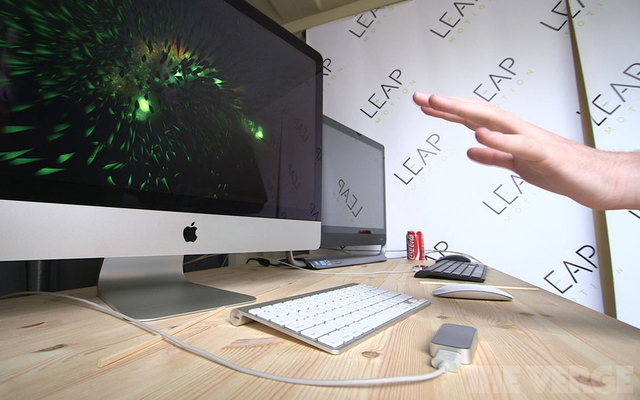
\includegraphics[ height=0.5\textwidth, width=0.65\textwidth]{leap-exp-watermark-rm-vrg_large_verge_medium_landscape}
\caption{Interacting with the LeapMotion \cite{theverge} }
\label{fig:leapmotionpicture}
\end{figure}

\section{LeapMotion}

The LeapMotion is a small device slightly larger then a USB drive which sits in front of a monitor and captures motion in 3 cubic feet of space using a pair of cameras. The small cameras triangulate the positions of hands, fingers and tools in their relative space between the LeapMotion and the monitor relaying accurate position and velocity data in real time. The data can then be used to control application by driving the user interface of the system \cite{leapmotion}. 

This type of interaction with the computer system is different from the traditional keyboard and mouse because it does not require any physical contact with objects connected to the system and has the ability to sense a much wider range of input. The LeapMotion is also expressive in three dimensions as opposed to two.

\begin{figure}
\centering

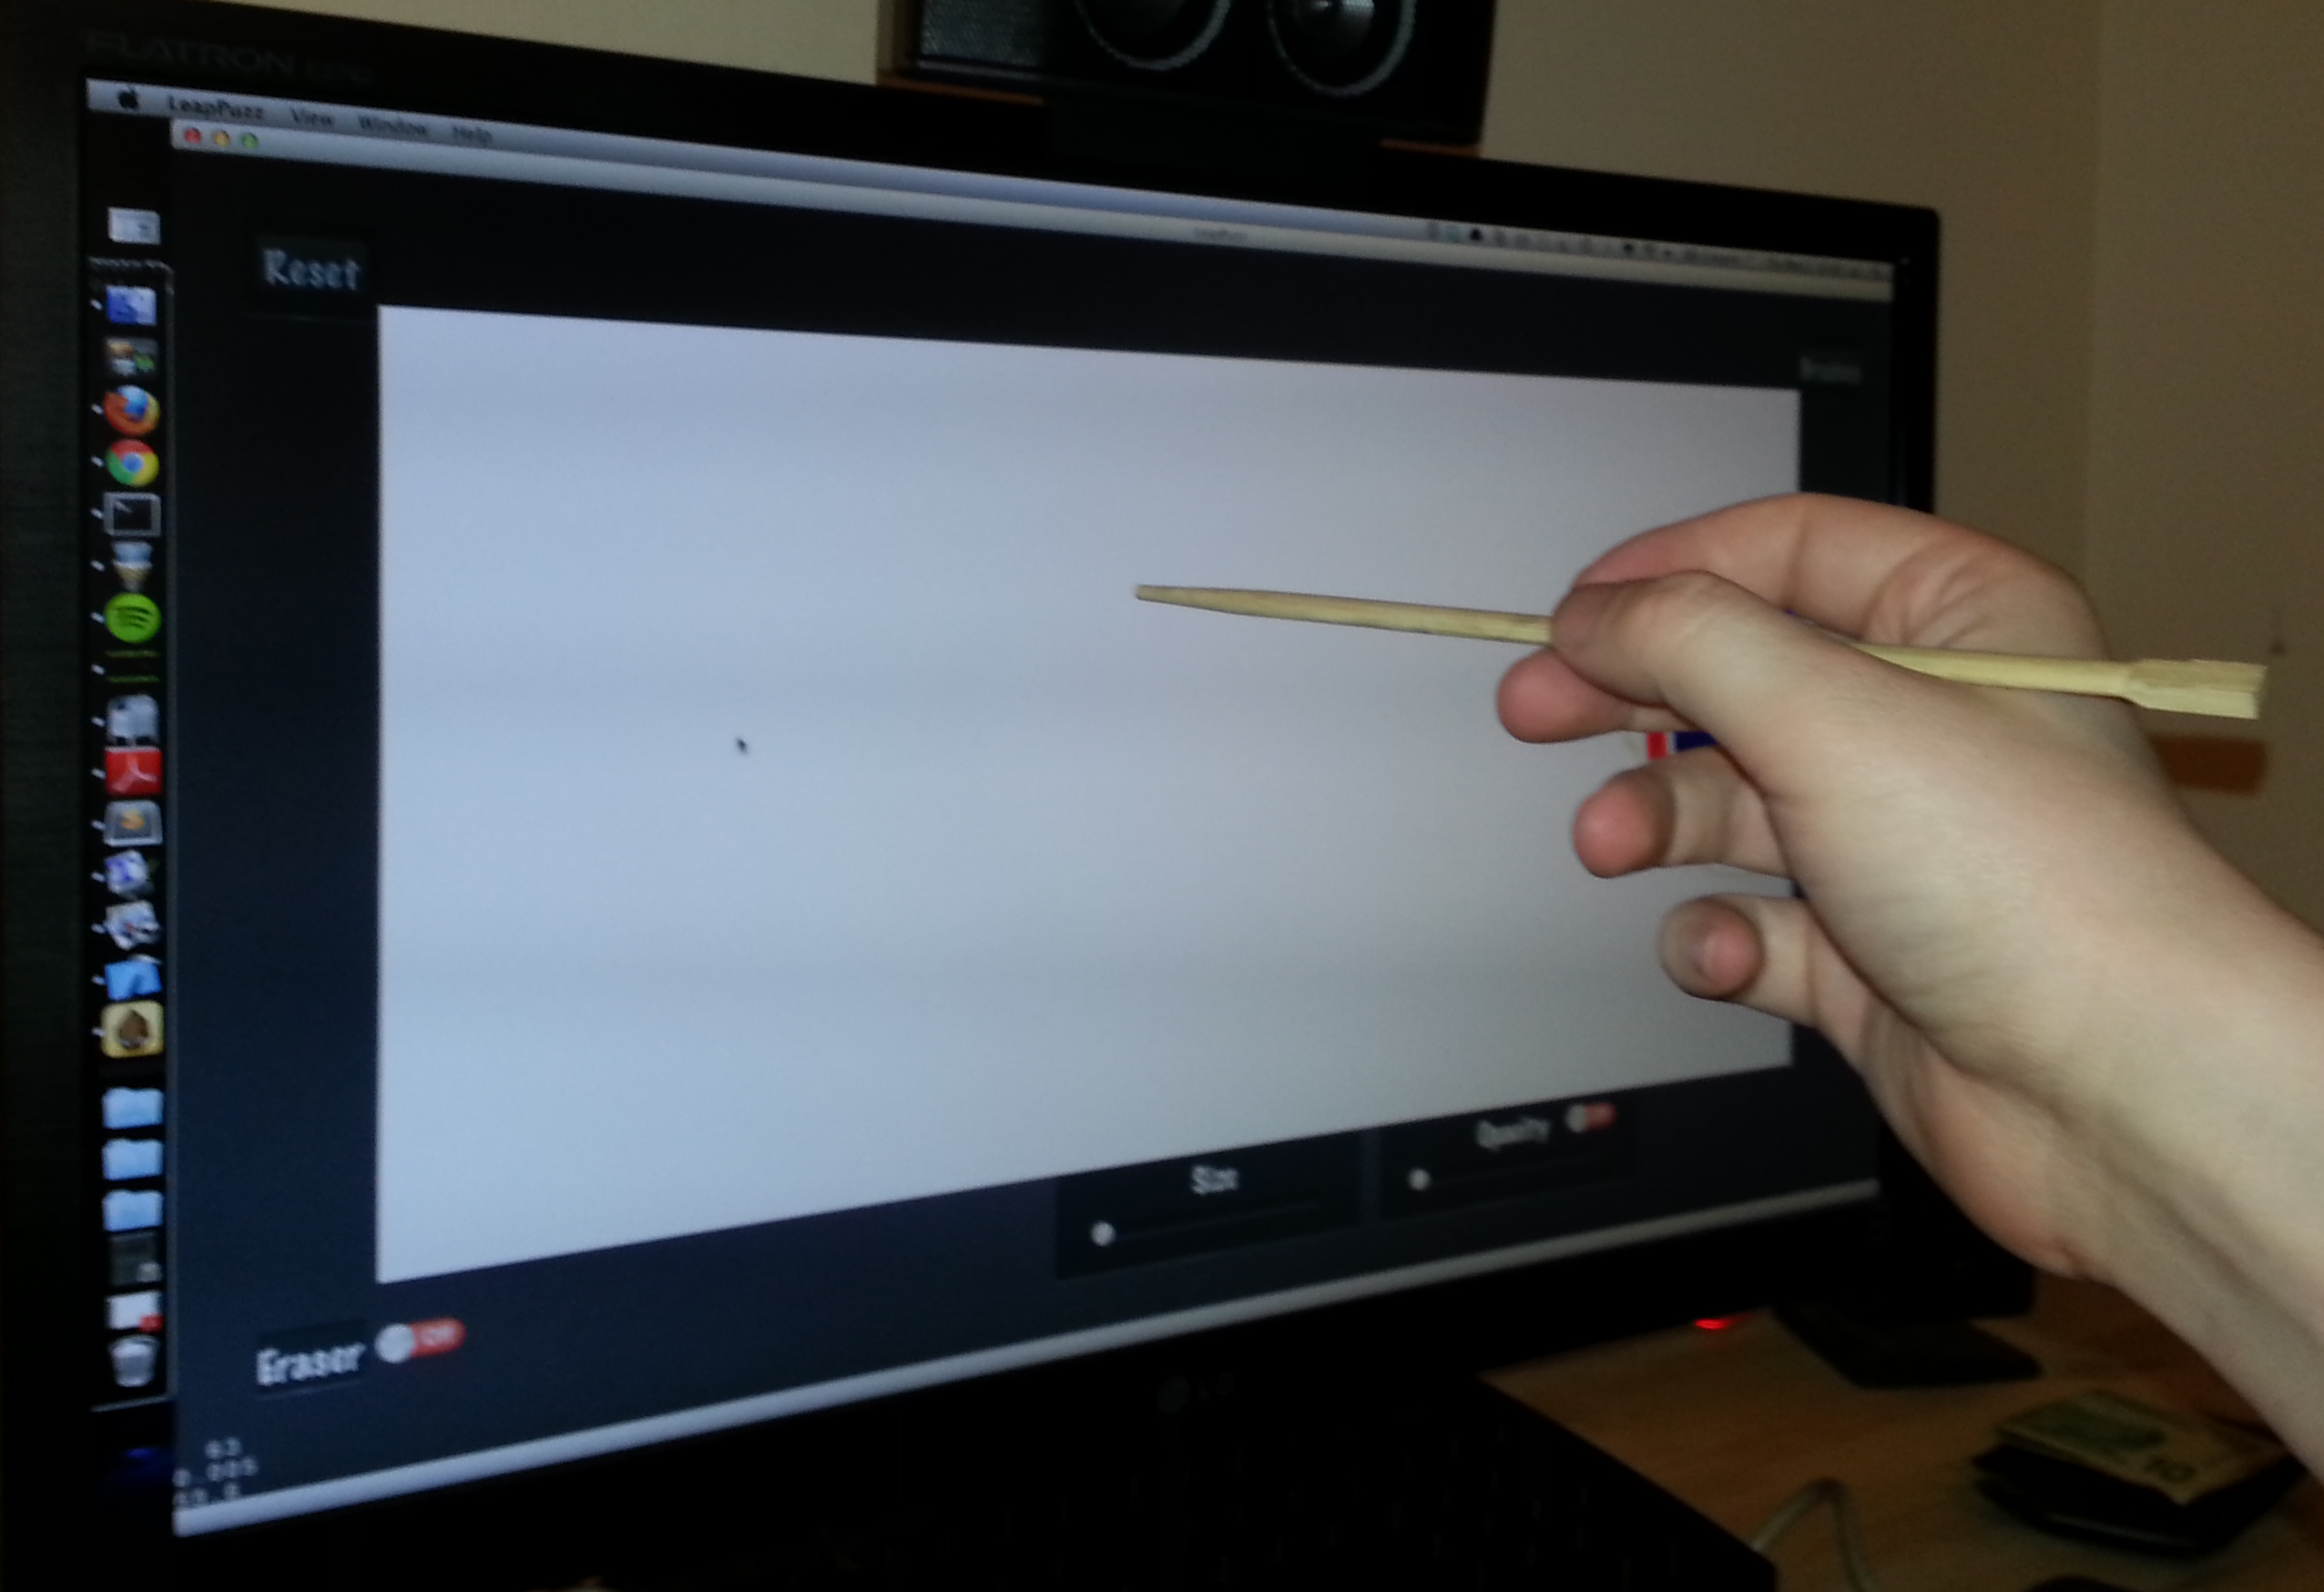
\includegraphics[ height=0.5\textwidth, width=0.75\textwidth]{chopstick}
\caption{Using a chopstick as a pointer}
\label{fig:chopstick}
\end{figure}
In this paper and throughout the project we refer to a finger or tool interacting with LeapMotion as a "pointer\footnote{The documentation refers to this as a "pointable"}." The tool can be any object is "stick-like" such as a pen, pencil or chopstick. Throughout this project a chopstick was mostly used as seen in Figure~\ref{fig:chopstick} as the preferable tool.

\section{Use Case Exceptions}
Although we wanted to see if the keyboard and mouse could be replaced by the LeapMotion there are some functions that we understand would almost be certainly not possible. Tasks that require the user to type large amounts of information, such as data entry or word processing, are two such examples of this exception. The focus, therefore, would be on some of the other functions the keyboard may serve such as switching applications which can be performed by the keyboard shortcut ALT + TAB or with a mouse. The LeapMotion might be able to replace this functionality with a wave of a hand indicating to switch the applications automatically in carousel. 


% Chapter 1

\chapter{Development Methodology} % Main chapter title

\label{Chapter2} % For referencing the chapter elsewhere, use \ref{Chapter1} 

\lhead{Chapter 2. \emph{Development Methodology}} % This is for the header on each page - perhaps a shortened title


This project differed from traditional software development projects in that it worked closely with children participating in the design process of the application. The project worked closely with a group called KidsTeam. The children affiliated with this particular group participated in the application's design process. Because of this collaboration, the project's development process was different from the traditional projects in the way the phases were performed and required a very flexible model of development. 

\section{KidsTeam}
The KidsTeam is a group of eight children ages 6 to 11, male and female, overseen by Dr. Jerry Fails at Montclair State University. The group met twice a week for one hour sessions over the course of a semester. During that time, the KidsTeam worked on various projects which were facilitated by Dr. Fails along with several undergraduate and graduate students.  The objective was to use the children's natural capacity for divergent thinking in order to study and identify new ways of collaborative learning and development as a means of designing a fun educational game to help elementary and middle school aged students learn and practice basic math skills. In order to achieve an optimal outcome, the professor and students created a community of respect and rapport. The purpose was to create a safe space where the children felt free to explore and share their ideas. Therefore, it was imperative that the atmosphere remain relaxed. This was enforced by rules that framed particular behaviors such as encouraging the children to speak when they have a thought, idea, or question rather than raising one's hand. The only strict requirement of the children during the sessions was that they must respect everyone, including the adults, in KidsTeam. 

KidsTeam creates a dialog when designing and developing an application between the developers and the users by building off each others ideas. This intergenerational design team collaborates by exchanging ideas and giving opportunities to enhance every aspect of the application. 


\section{Collaboration Techniques}
Several techniques were implemented in order to aid the development process. These techniques were chosen for their means to foster a community of cooperative inquiry where the children felt encouraged to contribute design ideas freely. \cite{journalsjcalScottMI03}\cite{Colella98}

%These techniques are designed to encourage children to freely contribute while divergently thinking to contribute design ideas. \footnote{Out of Our Minds}

\subsection{Sticky Notes}\label{sec:stickynotes}

\begin{figure}
\centering
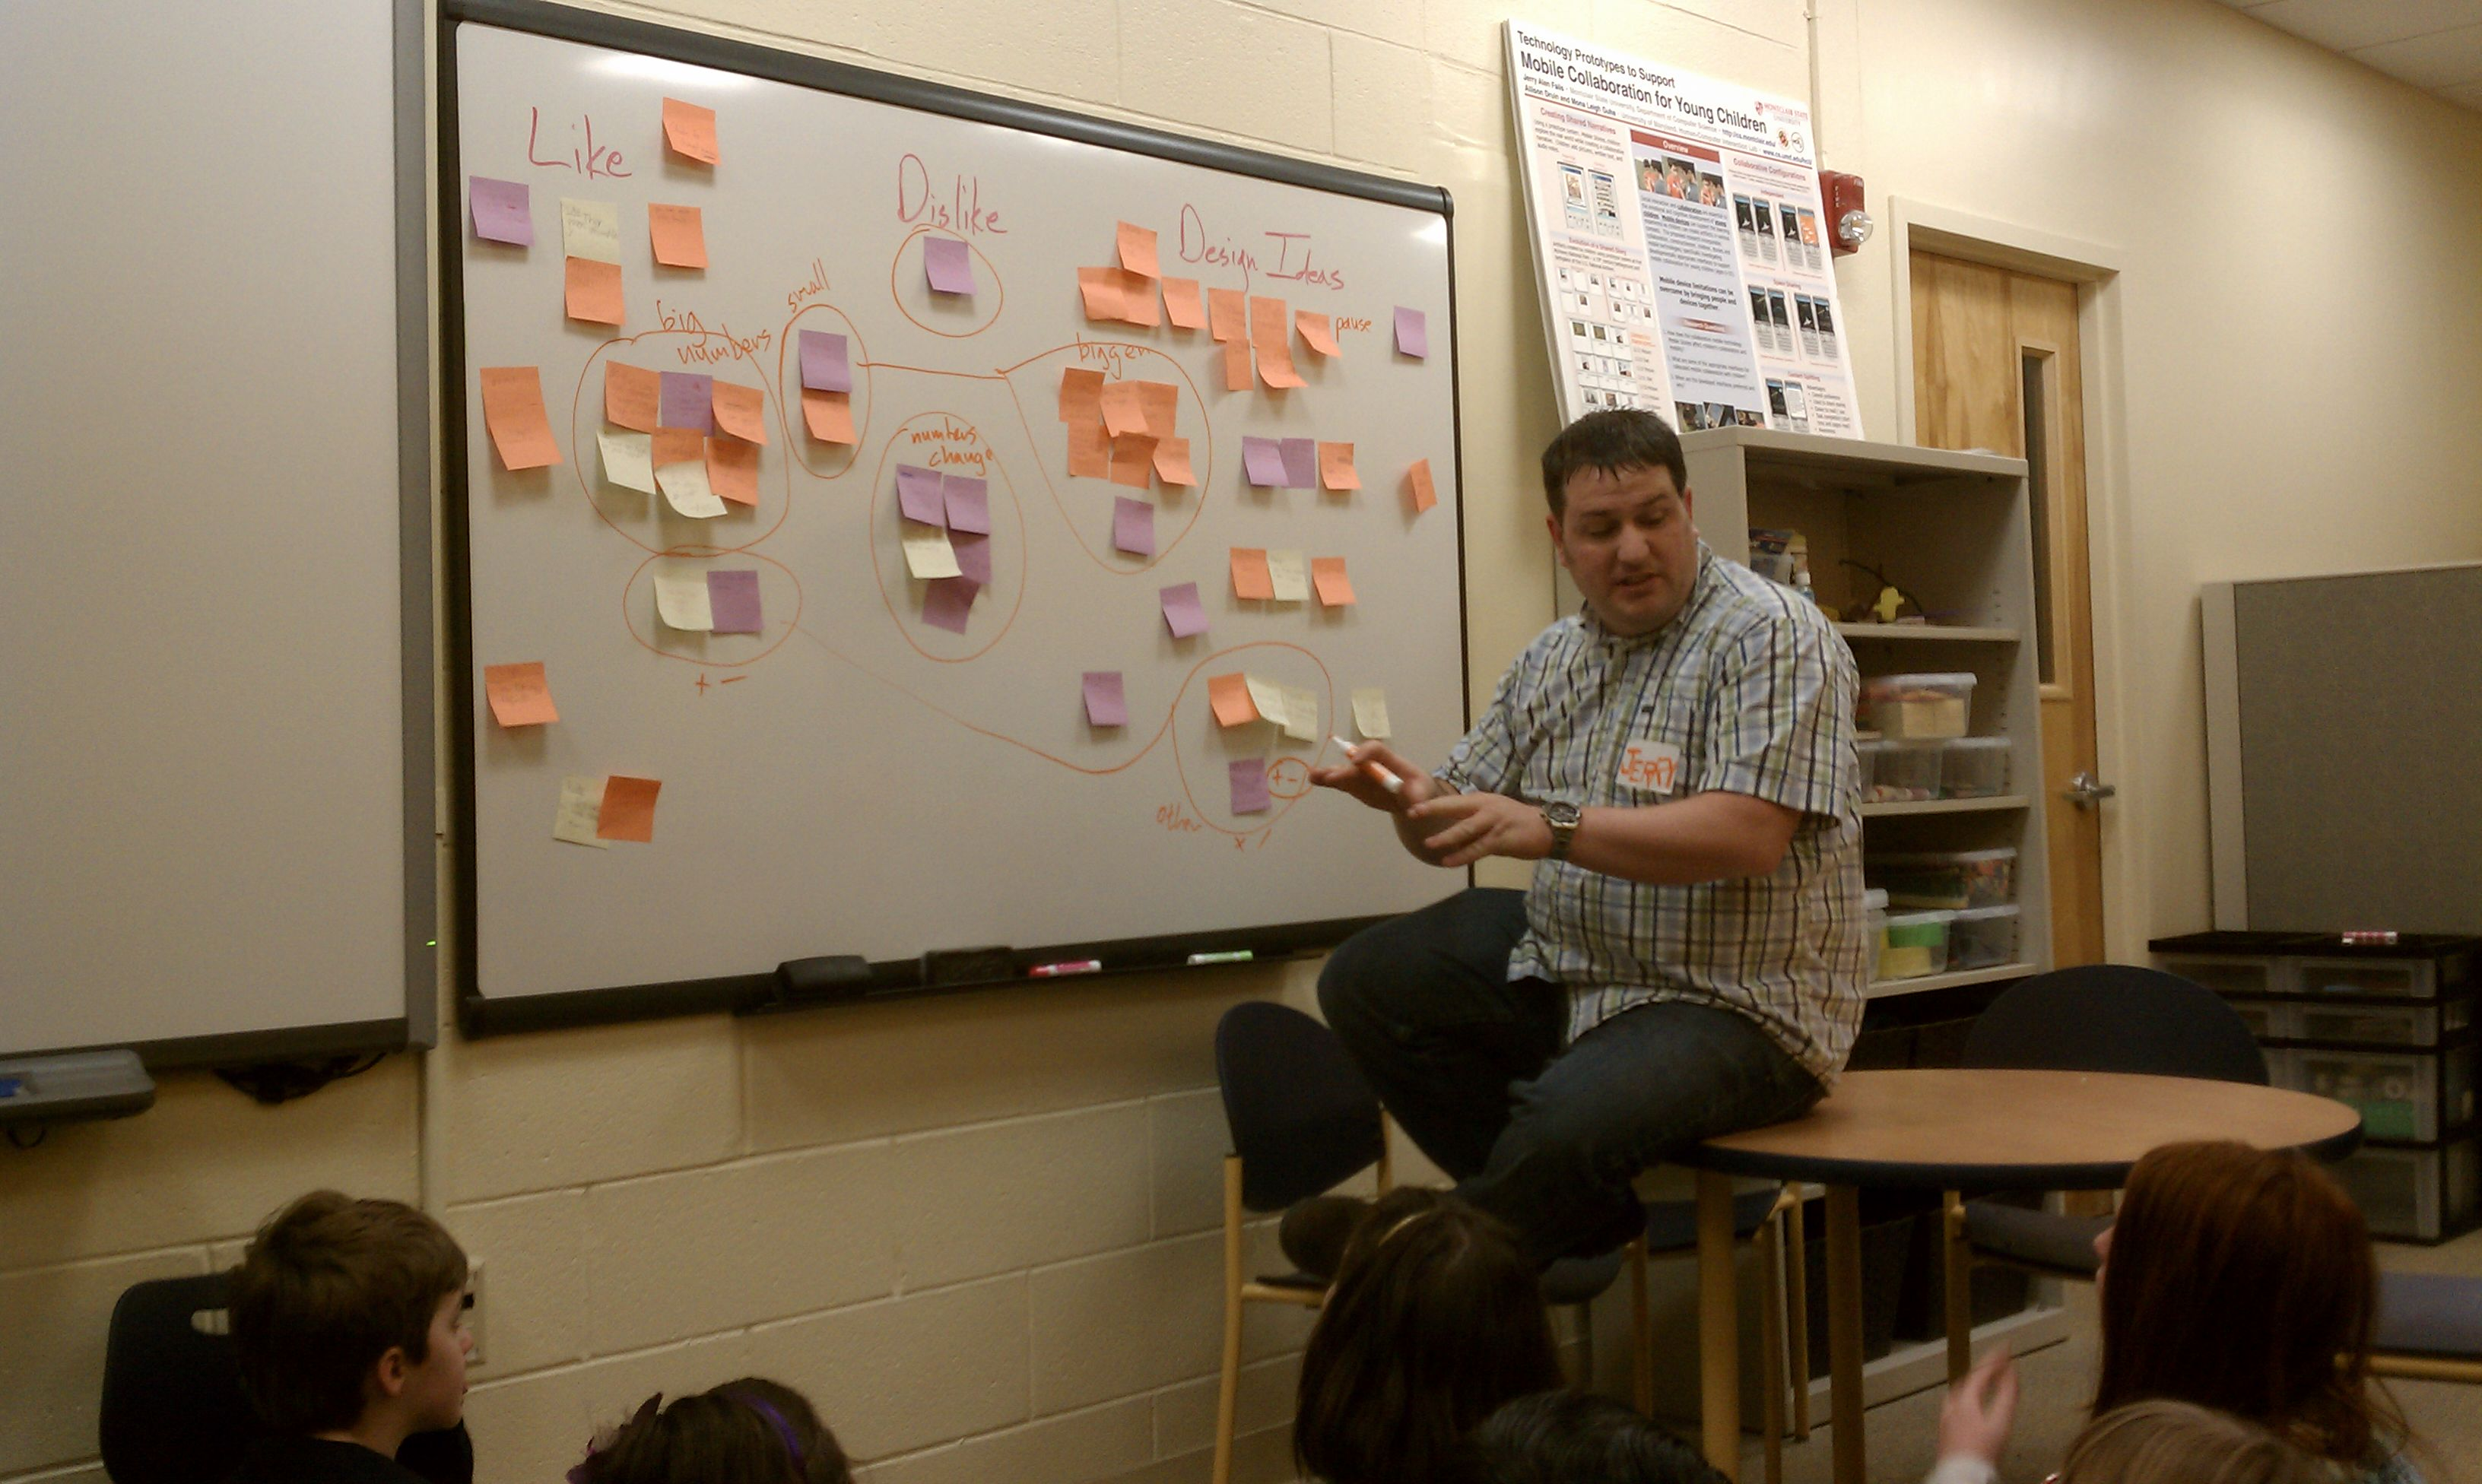
\includegraphics[height=1in, width=1.5in]{IMAG0270}
%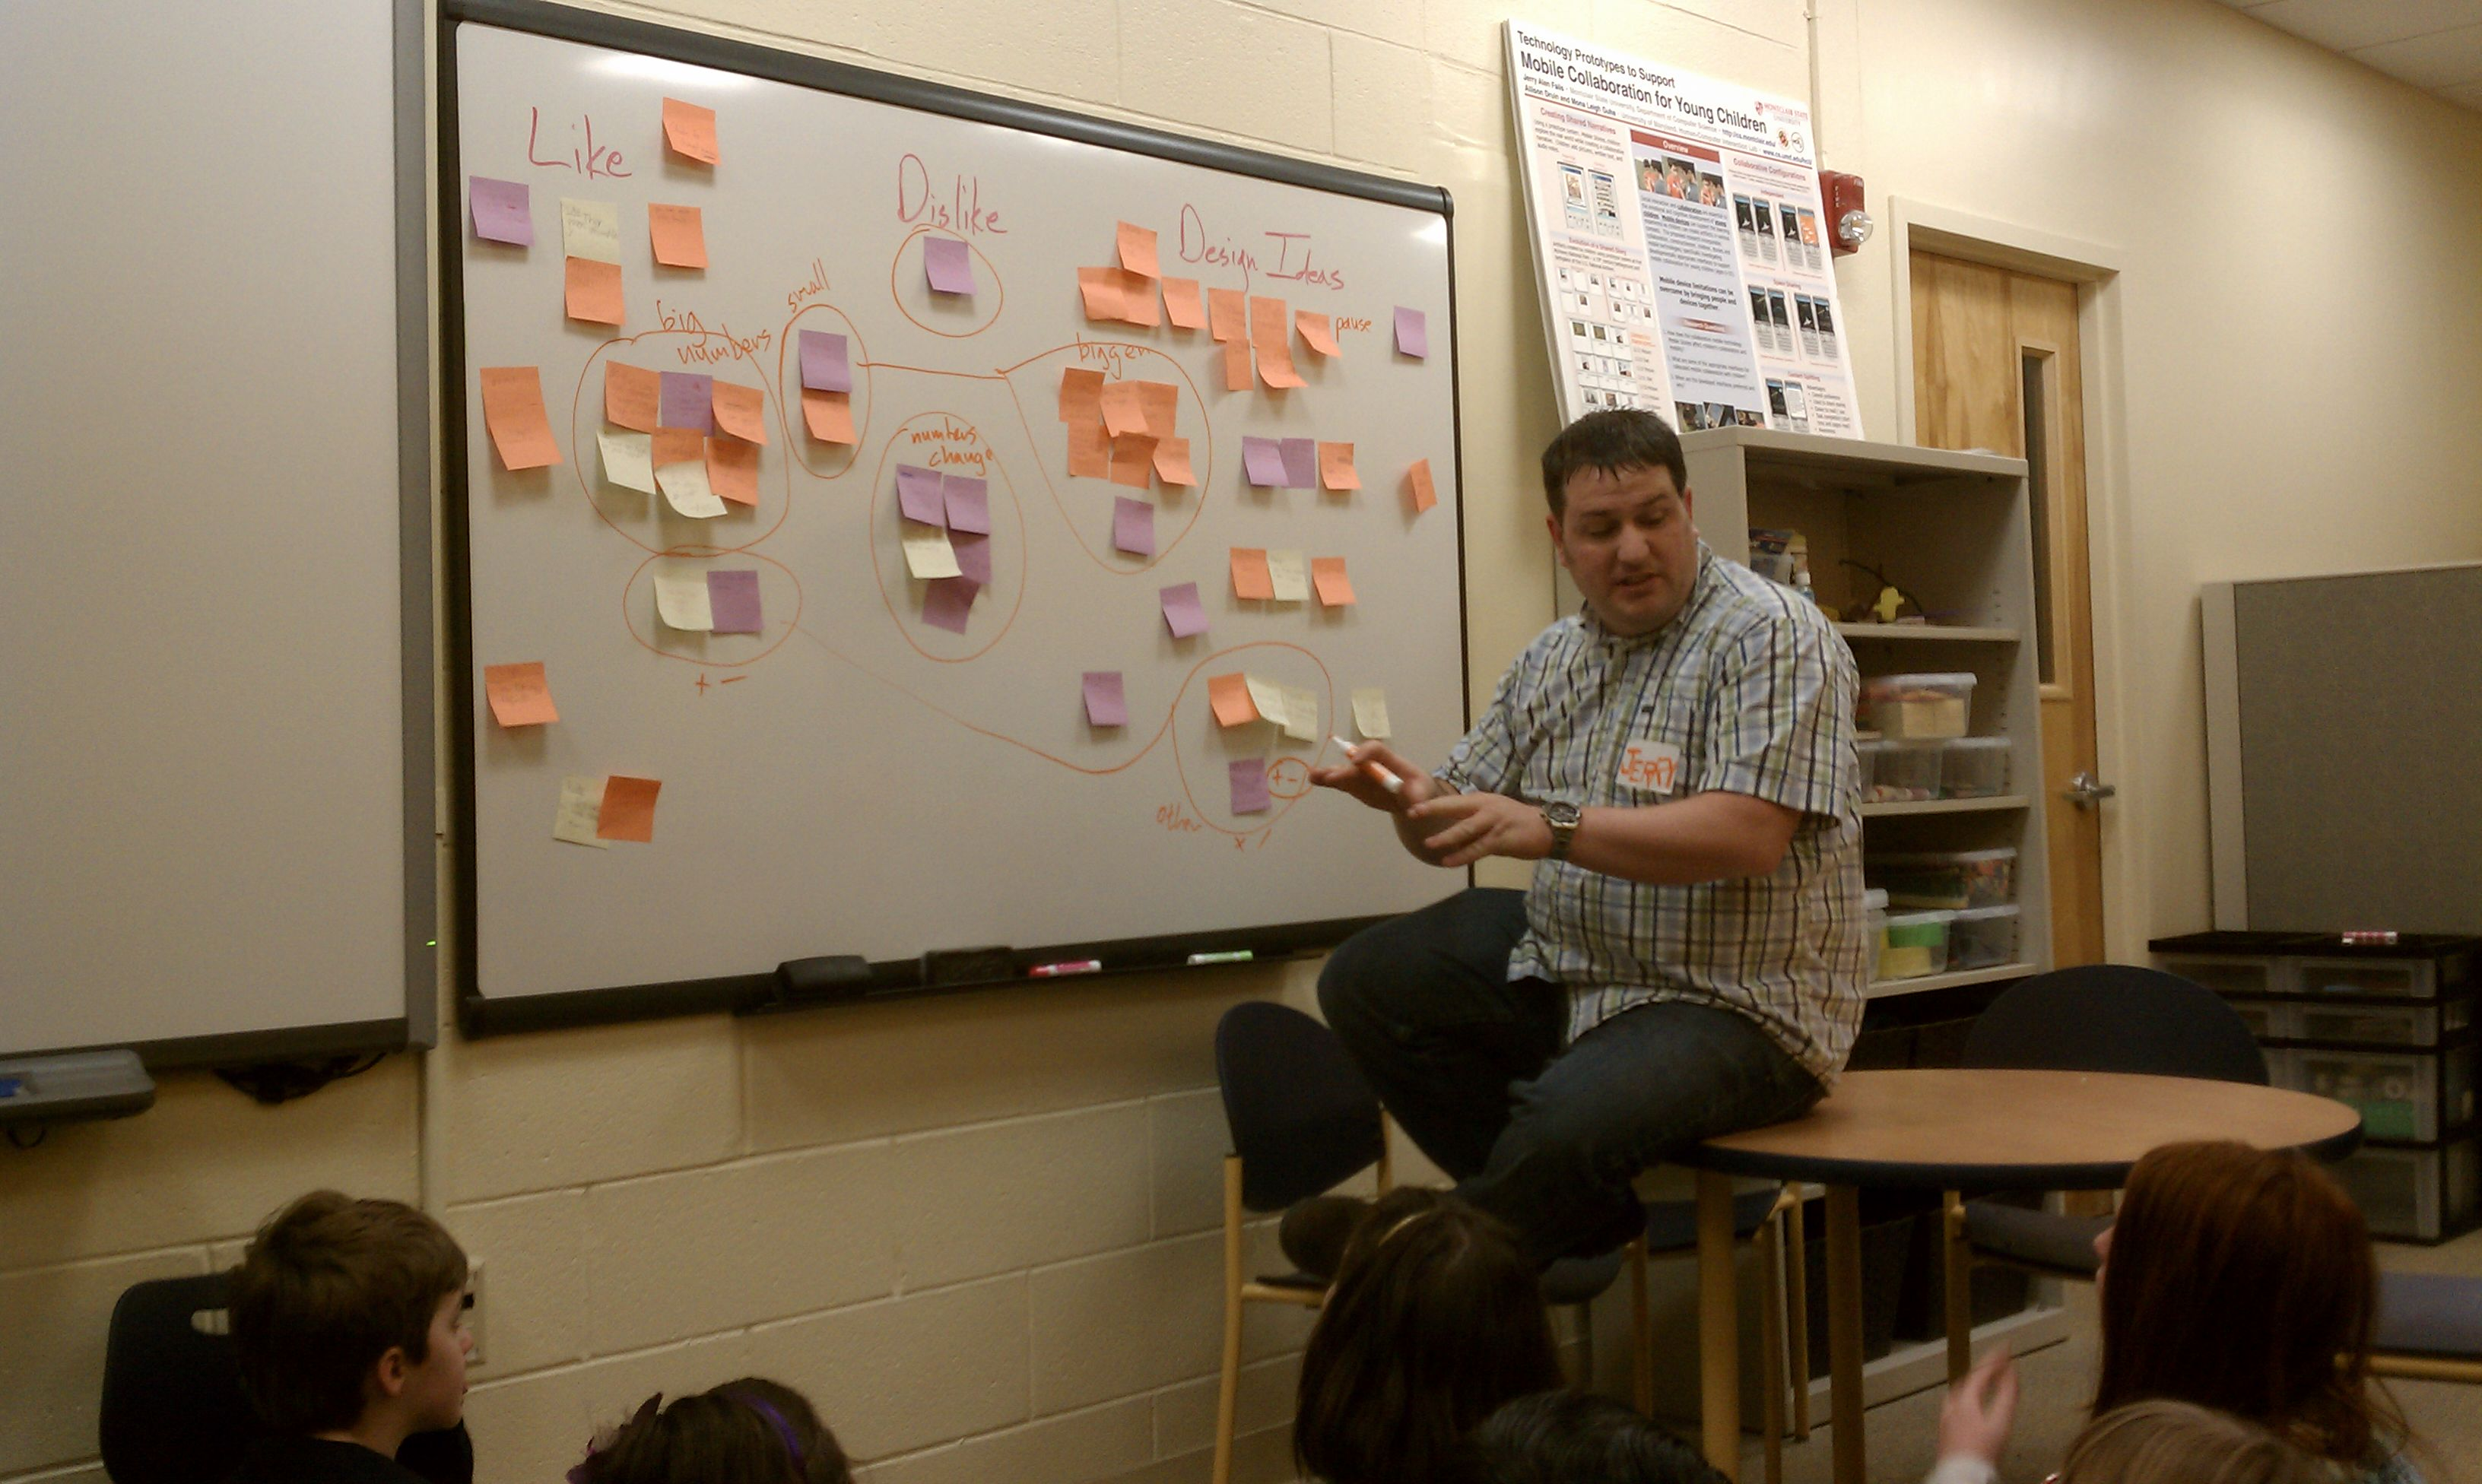
\epsfig{file=IMAG0270, height=1in, width=1.5in}
\caption{Reviewing the sticky notes using a spatial graph on a white board for easy comparison and analysis. }
\label{fig:stickynotesreview}
\end{figure}

Each child was given a pad of Post-It notes\footnote{Small square of paper with adhesive on reverse side.}.During activities which required comment, as the children played with the cubes, the children would write comments on the PostIt notes\footnote{One comment per sticky note.}. These comments were categorized into like, dislike, or design idea and then stuck to the white board. A facilitator would then organize the notes based on the category and the comment content to resemble a spatial graph where similar comments are grouped closer together, while outlying comments are spread farther apart. Comments relating to a specific function or component are arranged into the same row while the category of the comment will determine the column. At the end of the session the observer debriefs with the children about the session by reviewing the comments arranged on the white board and having the children comment about the session overall. This time allows for the observer and the children to summarize the session, gives the children extra time to comment and provide more specific feedback, and permits the observer to further clarify a child's reasoning for making certain comments. The result is a frequency analysis as seen in Figure~\ref{fig:stickynotesreview} which feedback can be turned into specifications for the next design cycle.  \cite{Druin:1999:CID:302979.303166}\cite{Druin02therole} 

\subsection{Bags of Stuff} \label{sec:bagsofstuff}
Each child is given a Bag of Stuff that contains a variety of arts and crafts supplies such as Popsicle sticks, felt, construction paper, markers, etc. The children are then given a design concept by the observer and asked to use these materials to construct that concept. As the children build, they must explain in their own words how their concept works while the observer takes notes. \cite{Druin:1999:CID:302979.303166}\cite{Druin02therole}

\subsection{Storyboarding}\label{sec:storyboarding}

The children are split into groups. The groups were chosen at random and did not remain intact from session to session. Each group then receives one large piece of construction paper. They will use the paper, sticky notes, and markers to draw their particular game concept sequence of events. Any actions or changes in a scene must be drawn in the order that they occur. The children must use arrows to delineate the progression of events. In order to make sure their ideas are conveyed clearly, the children are asked to be as descriptive as possible while facilitators take notes as the children work. \cite{Druin:1999:CID:302979.303166}\cite{Druin02therole}

\section{Development Model}
Working with KidsTeam required a lot of flexibility in the development process and is why Rapid Application Development (RAD) model\footnote{Iterative or incremental development process resembling an evolutionary pattern.} for software development was chosen as the best fit model for this project. The RAD model uses rapid prototyping\footnote{Rapid Prototyping is a quick mockup for testing} and continuous iterative cycles which allowed for testing with KidsTeam on a weekly basis. Each session with the KidsTeam generated new requirements and fixes to be implemented within tight time constraints prior to the next session.

\subsection{Specification}

\subsection{Design}

\subsection{Code}

\subsection{Test}

\subsection{Review}

%Maybe you can fluff this section by defining what each of the terms mean, such as defining "specification" "design" so on and so forth.

The model centered around five phases Specification, Design, Code, Test and Review as seen in Figure~\ref{fig:agiledesignprocess} constituting a full cycle. Changes in the specification were then implemented and reflected in the application prototypes ready for the next session. Each session with KidsTeam marked the end of current cycle and start of the next in the development process. \cite{0136061699}\cite{Ruparelia:2010:SDL:1764810.1764814}

The children were most heavily involved in the specifications, design, test and review phases in each of the nine sessions. Some parts of the design and testing were done independently of the children but mostly elaborated either on their designs and ideas or were performed to ensure the application was stable enough for testing with the children.  

%Agile foot note and reference if it can be included  K. Reed, E. Damiani, G. Gianini, and A. Colombo.
\begin{figure}
\centering
%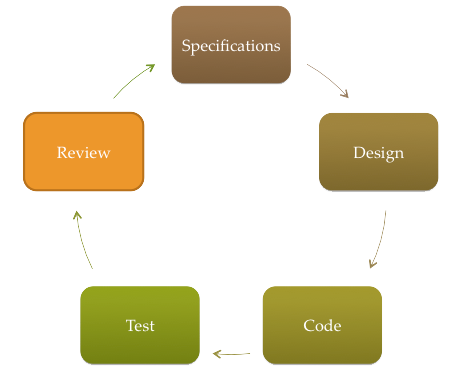
\epsfig{file=agiledevelopment2, height=0.95\columnwidth, width=\columnwidth}
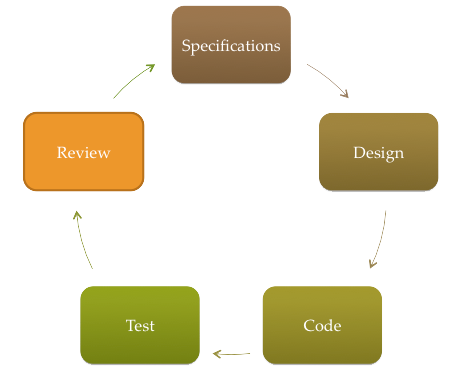
\includegraphics[height=0.5\textwidth, width=0.5\textwidth]{agiledevelopment2}
\caption{Rapid Application Development cycle }
\label{fig:agiledesignprocess}
\end{figure}


\section{Progress Updates}
%Done via the wiki and Youtube updates 
% Chapter 1

\chapter{Design and Development} % Main chapter title

\label{Chapter3} % For referencing the chapter elsewhere, use \ref{Chapter1} 

\lhead{Chapter 3. \emph{Design and Development}} % This is for the header on each page - perhaps a shortened title

%----------------------------------------------------------------------------------------

%\subsection{Goals}
%\subsection{Observations}
%\subsection{Outcomes, Developments and Improvements}


%Throughout the project nine session were spent The initial sessions centered around introduction of the LeapMotion exploring how it could be used with existing interfaces and designing new interfaces. In the later sessions the application and interface begin to take form and requirements will begin to solidify. 

Throughout the project nine session were spent with KidsTeam. The initial sessions with the KidsTeam centered mostly around the introduction of the LeapMotion. The purpose was to help the children become comfortable with the technology through both brief explanation of how it works and independent exploration. It was important that the children spent time interacting with the technology as early on in the sessions as possible. The more comfortable the children were with using the LeapMotion, the more realistic their creations could be for the interface. 

Later sessions focused on reviewing and improving the application. The application will not be able to make too many drastic design or architectural changes in these later phases.
%Febuary 5th
\section{Session 1: Introduction and Brainstorm}\label{session1}

This first session with the children started with brainstorming ways to use a computer system or control an application without a keyboard and mouse and only using their hands. Using the Bags of Stuff~\ref{sec:bagsofstuff} exercise the children explored designing applications that could only be controlled using gestures.

The children developed several application and game ideas including Pong, Fruit Ninja, Temple Run, Virtual Pet, Internet Explorer, Paint and Maps. The applications were accompanied by many controlling gestures such as a chopstick with button, waving, grabbing, pointing, dragging, pull and release\footnote{Similar to the bird launching interface in Angry Birds}, scratching and striking. 

Afterward the children were allowed to play with a LeapMotion visualizer of the LeapMotion at the end of the session. The visualizer is 3d rendering of what the LeapMotion detects in realtime. 

%\subsection{Goals}

%\subsection{Observations}

%\subsection{Outcomes, Developments and Improvements}

%Feburary 12th 
\section{Session 2: Testing Breakout and Designing a Paint Application}\label{session2}
The children tested a simple BreakOut game which allowed them to interact with the LeapMotion with an application and get a feeling of how it works. With that experience the children were then tasked with designing a painting application that can draw, choose colors and brushes only using gestures to control the interface of their application using the storyboarding~\ref{sec:storyboarding} technique. 

Along with the interface the children came up with several gestures in controlling a variety of user interface controls but most of the gesture controls relied on techniques similar to the way a mouse would function in picking up, dragging and dropping an icons on the screen. Other designs required an action to be performed while pointing at the targeted user interface control indicating a beginning action or ending action\footnote{begin and end actions} instead of waving of a hand, drawing a figure eight in the air or a slashing motion. 

\section{Gesture Design Challenges}
The immediate challenge that faced gestures requiring beginning and ending triggers is how to interpret when each trigger takes place to perform the action. In the mouse and touch screen interfaces the typical design paradigm consists of a beginning action, intermediate action and ending action respectively representing the state in which the input is currently in.

\begin{center}
\captionof{table}{Apple Mac OS X and iOS Application Programming Interface for standard methods of input \cite{appleapi}} \label{tab:title} 
    \begin{tabular}{ | l | l | l |}
    \hline
    Action & OS X & iOS \\ \hline
    Begin  & MouseDown & TouchesBegan \\ \hline
    Moved & MouseDragged & TouchesMoved \\ \hline
    End & MouseUp & TouchesEnded \\ \hline
    Alternate & -- & TouchesCancelled \\ \hline
    \end{tabular}
\end{center}

With the LeapMotion there was no standard way of detecting when each action is to be performed. With this challenge the children came up with the concept of using two fingers to indicate when an action would be performed. Using the thumb as the control mechanism to indicate the action state to be performed and the index finger to indicate the targeted interface control to act upon, the interface control could triggered based on its functionality. The gesture consisted of pulling the thumb flush to the hand while pointing at the user interface control to begin the action and releasing the thumb to indicate the end of the action.With this simple system the a gesture could perform a BeginAction, MovedAction, and EndAction on user interface controls. 


\begin{figure}
\centering     %%% not \center
\subfigure[Open Thumb]{\label{fig:a}
\includegraphics[width=60mm]{HandPointOpen}}
\subfigure[Closed Thumb]{\label{fig:b}
\includegraphics[width=60mm]{HandPointClosed}}
\caption{Hand trigging actions}
\end{figure}

Use case include some of the following control operations

\begin{itemize}
\item Icon Movement pulling the thumb flush to the hand would trigger the BeginAction "pickup" the icon and start dragging it on the screen. The icon could then be placed anywhere on the screen until releasing icon and "dropping" at that position by moving the thumb to a relaxed position no longer flush with the hand performing the EndAction.
\item Selecting a color. The BeginAction would present a popover that would remain open while the user pointed at the desired color until the EndAction. The EndAction would select the color that was pointed at when triggered. 
\item Radio Buttons. A quick BeginAction and EndAction trigger while pointing at the radio button would change the state of the selected item. 
\end{itemize}

\subsection{Implementation Challenges}
In concept this idea seemed to be an ideal and natural way of interacting with the system but faced several challenges. When the thumb became flush with the hand the LeapMotion could no longer detect it as a finger. Additionally, there were several instances of occlusion occurring, for example when the hand was positioned with the thumb pointing upward the line of sight from the camera to the thumb was blocked. This unique challenge was difficult because the thumb could not be accounted for in all cases. An option might be to use the thumb's absence as a trigger although this is prone to many false positives\footnote{False positive indicates a given condition is present when it is not.} when the user's hands were on the boarder line of the LeapMotions visibility range or has lost track of the thumb due to occlusion\footnote{Occlusion occurs when the a surface is hidden by blocking the line of sight.}. Reversing the actions and performing the opposite gesture did not feel natural. Holding the thumb closely to the rest of the hand is not relaxed state and also did not mimic the act of grasping something or triggering an action as people are more commonly used to. 


\subsection{Unity 3D Engine Testing}
Touching two or more fingers together rendered them not recognizable by the LeapMotion and thus would not allow pinch gesture to be used. Alternatives might be calculating when two fingers are close to each other although the LeapMotion cannot differentiate the fingers into which is the index, middle, ring, pinky, and thumb fingers. The application would have to assume any two fingers were performing the gesture and would not allow for the natural separation between fingers unless all fingers were kept folded tight into the hand until needed. 

To observe this behavior a separate project was setup using the Unity 3D Engine to track the different pointers and their interactions in 3D space.\cite{unity}

It was clear after some lengthy prototyping and testing that some of the gestures developed by the children would not be possible and also raised some preliminary speculations that the LeapMotion may only be supplemental in its role except when in application specific situations. Different methods of interacting with these types of controls would need to be developed or would rely on the keyboard and mouse for their functionality.

%%%%%% --- section end

%Feburary 19th
\section{Session 3: Interface Controls}\label{session3}

Common user interface controls were printed out and the children were tasked with brainstorming how they might use LeapMotion to control the widgets or design their own widget that can reproduce the functionality. The user interface controls that we focused on included performing the following tasks were: buttons, drop downs, color palettes, check boxes, radio, buttons, sliders, toggles, steppers, wheels, trees and tabs.

%The user interface controls that have become common and standardized in almost all computer system would need to be adapted or changed to work with the LeapMotion. 

%The user interface controls that required direct text entry would be excluded due to the use of the keyboard although we could not disregard some of the shortcuts that a keyboard provides. In some systems when selecting from a list the keyboard provides a short cut for selecting an item. For example when selecting a the "NJ" for a list of state abbreviations pressing the "N" key will jump to the N section and pressing it repeatedly will cycle in alphabetical order through all of the items starting with letter "N". 
\begin{figure}
\centering     %%% not \center
\subfigure[Carousel view style]{\label{fig:car}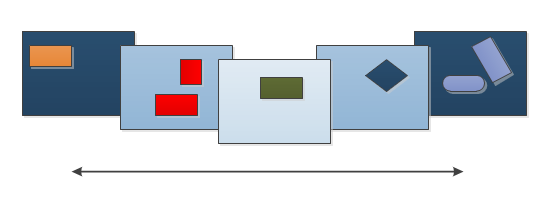
\includegraphics[width=60mm]{car}}
\subfigure[Collection view style]{\label{fig:pan}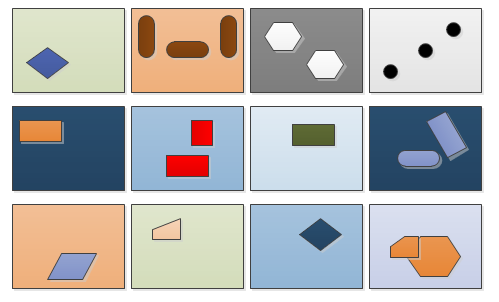
\includegraphics[width=60mm]{pan}}
\caption{Carousel view style maybe zoomed out using a pinch and pull gesture to a collection view. }
\label{fig:collectionview}
\end{figure}
The children did not come up with many new ways of interacting with the user interface controls or developing their own. The main method of interaction focused on pointing to the interface control triggering it using a hand signal with their fingers. The wheel controls could be controlled with flicking motions and dialogs could be dismissed with a wave indicating that the user is finished with the form. Selecting from a list could be done with a list in a carousel view style~\ref{fig:car} where each of the items could be panned through by waving or zoomed out into a collection view style~\ref{fig:pan} of items using pinch and pull gestures. 

Observation of this session reinforced the suspicion that the LeapMotion may not be able to take a role as a dedicated device but as a supplemental device to the mouse an keyboard. Interface controls would also require more space between each of other and to be a of a larger size allowing for a margin of error. Feasible options may include iOS style of modal dialogs which take primary focus until the user in completed with the control. 

%Feburary 26th
\section{Session 4: Testing a drawing application}\label{session4}

Demonstration and hands on testing of a prototype drawing application developed based on the specifications the children had designed in the previous. The children provided feedback using the sticky notes exercise ~\ref{sec:stickynotes} review technique. 

The one requirement that stood out the most early on was the necessity for a Heads Up Display (HUD) which would track where the a pointer is pointing on the screen and also display and interaction with the pointer. Additional features might include motion streaks or gesture animations to provide visual conformation of the action being performed or help the user track where the pointer has been. 

%%Mouse trails paper citation?


%March 5th
\section{Session 5: Designing Gestures }\label{session5}

The children were given some sample gestures and asked to design a way of using the gestures or generate their own for using Microsoft Paint application using the storyboarding~\ref{sec:storyboarding} technique. The sample gestures were turning, tapping, swiping and hand wave. 
\begin{figure}
\centering

\includegraphics[height=1.5in, width=1.5in]{handbox}
%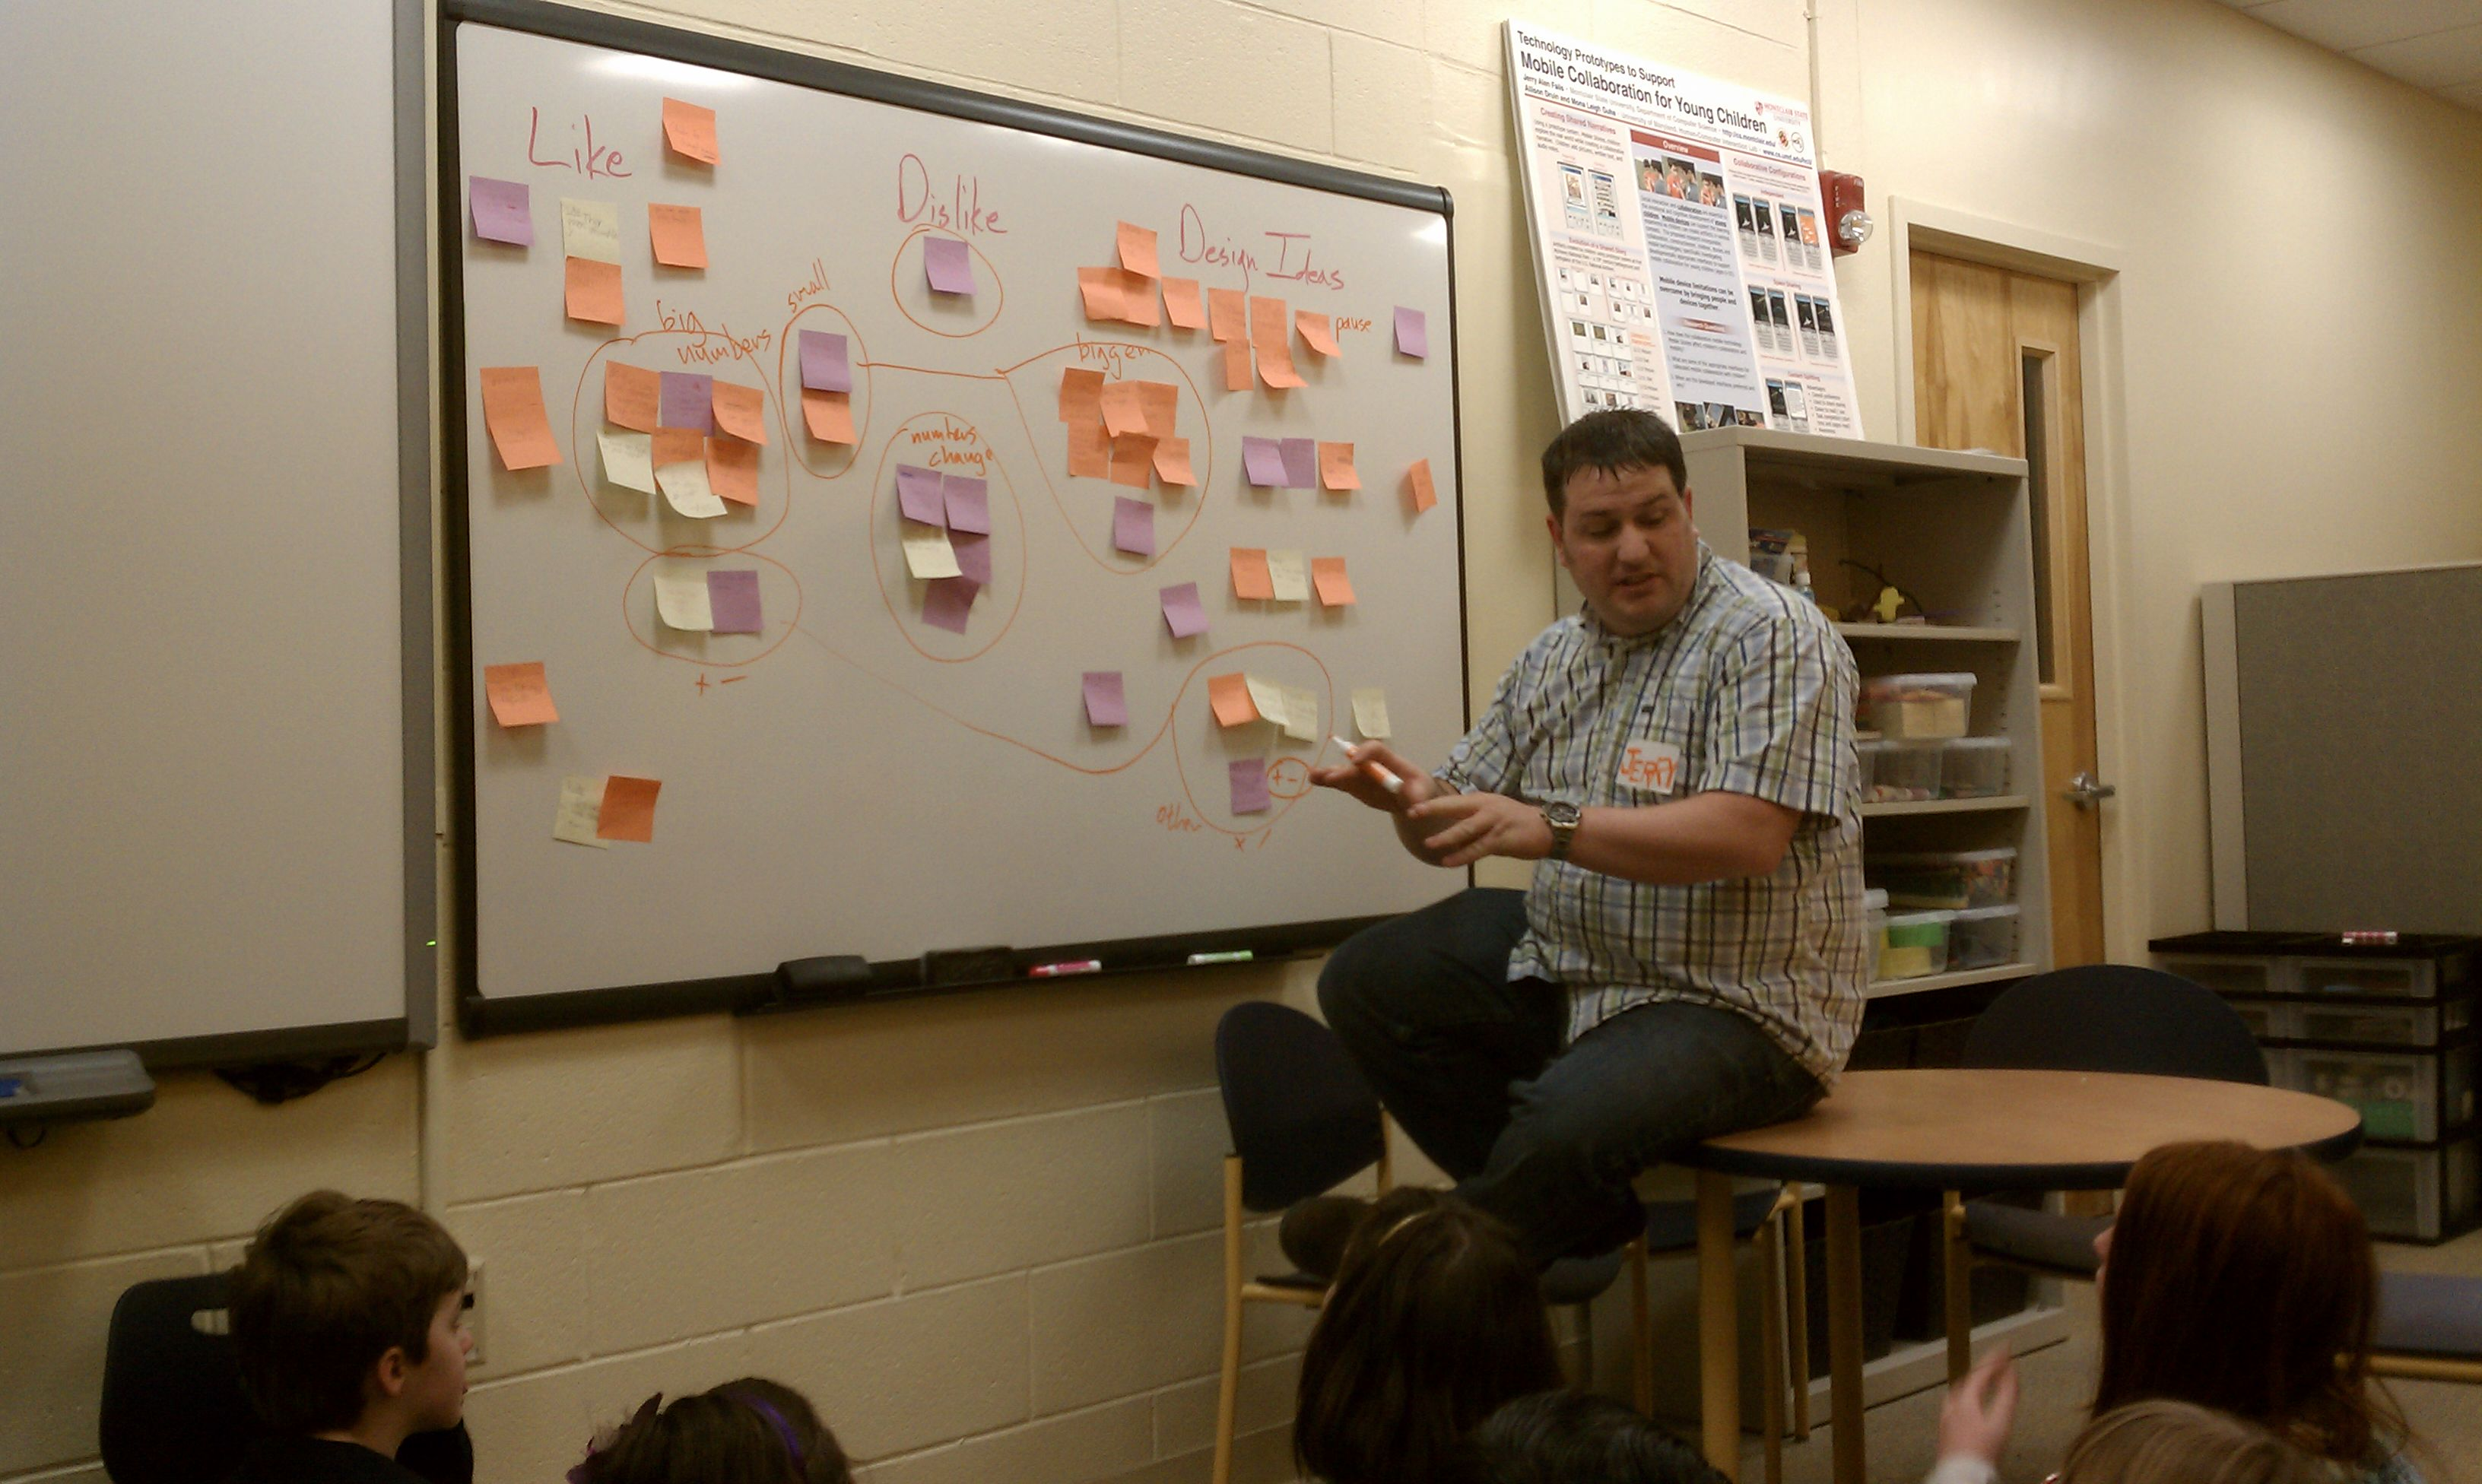
\epsfig{file=IMAG0270, height=1in, width=1.5in}
\caption{Indicating the size of a box by specifying two opposing corners with 'L' shape between the index and thumb fingers.}
\label{fig:handbox}
\end{figure}
Gestures developed by the children were fairly consistent to previous session in pointing to a user interface control and selecting it to perform the action. In the group discussion an idea to use two fingers on two hands to draw the bounds of the box was generated. The finger tips could either represent each of the four corners of the box or two opposing corners by making an 'L' shape as seen in Figure~\ref{fig:handbox}. 

This session reinforced the idea that the LeapMotion cannot be a dedicated device but a supplemental device.

%March 19th 
\section{Session 6: Testing Paint Prototype}\label{session6}


The children were tasked with testing the painting prototype application dubbed LeapPaint using the sticky notes exercise ~\ref{sec:stickynotes} review technique. This early prototype focused on adding a HUD to display the cursor and did not have all of the features in the initial requirements. Testing was focused on the interactions with the cursor. The While not testing they designed their own brushes, shapes and tools to be included in the next iteration of the tool. The overall consensus from this session was to implement better accuracy of the tool which required redesigning how the coordinate systems were translated from LeapMotion space into the application. 

%Go into coordinate systems here performing a vector  triagulation 

%April 2nd
\section{Session 7: Testing Improved Paint}\label{session7}


The children were tasked with testing the painting application with the fixes based on the last session and providing feedback using the sticky notes~\ref{sec:stickynotes} review technique. The new features focused on testing in the application were changing colors, erasing and an experimental method of triggering the drawing action. 

The two different drawing actions were tested with one using the space bar to indicate when to begin drawing. The other used the Z axis of the LeapMotion to begin drawing when breaking a certain plane of depth toward the screen. Children could switch between the modes by pressing the '1' key for space bar mode and the '2' for depth mode and compare each of them.

After testing the children noted that it was difficult to determine where the plane was that would start and stop the drawing actions using the depth mode. The space bar mode seemed to be the preferable option of the two. 

To help the children determine whether they were drawing or not a ring indicator would later be added to show when drawing and not drawing around the cursor by changing from green to red. Additionally the depth mode's flat plane along the Z and X axis would have to calculated as a concave shape for better performance since painting near the edges of the drawing required moving the arm slightly further toward the screen then required in the center. 
%%Figure for this if possible. 


%April 9th Testing and review of the application with sticky notes
\section{Session 8: Final Testing}\label{session8}

The children were tasked with testing the painting application for the last time using the sticky notes~\ref{sec:stickynotes} review technique. Testing for new features which included a depth opacity control. The opacity of the brush would become greater the closer the pointer was to the monitor simulating how a paintbrush or marker makes a darker line when pressed harder to paper. 

The children preferred the method of using depth to control the opacity over performing the manual adjustments with the mouse. 
\begin{figure}
\centering     %%% not \center
\subfigure[]{\label{fig:car}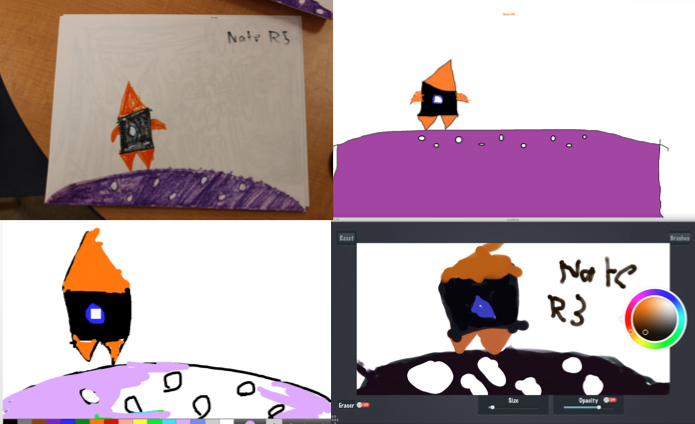
\includegraphics[width=60mm]{compare1}}
\subfigure[]{\label{fig:pan}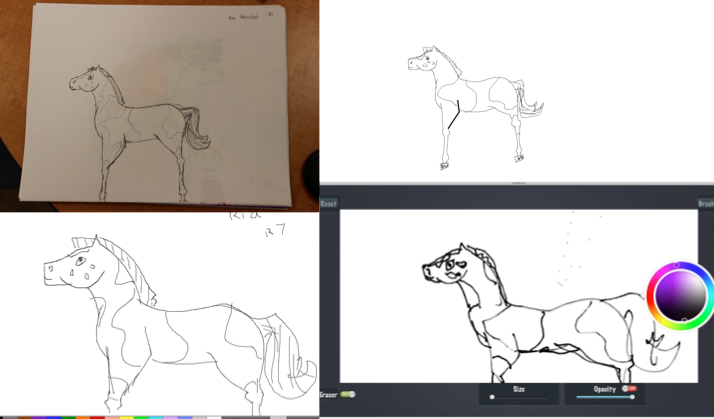
\includegraphics[width=60mm]{compare2}}
\caption{Drawings done by hand (top left), in Microsoft Paint (top right), on the iPad (bottom left) and with the LeapMotion (bottom right)}
\label{fig:comparisondrawing}
\end{figure}

%April 15th
\section{Session 9: Usability Comparison}\label{session9}
The last session compared the LeapPaint application with a three different methods of drawing with different interfaces. The children were given the task of drawing the same picture of their choice on each system. Each child was given 10 minutes of time to attempt to reproduce a drawing by hand drawing using markers, Microsoft Paint using a mouse and keyboard, SimpleDraw on the iPad's touch interface and with LeapPaint using the LeapMotion. 

The resulting drawings were mixed in comparison but showed that the drawing ability in the application may be related to the amount of time the child has had using the application. Drawing comparisons can be seen in Figure~\ref{fig:comparisondrawing} by two different children. 




% Chapter 1

\chapter{Application Architecture} % Main chapter title

\label{Chapter4} % For referencing the chapter elsewhere, use \ref{Chapter1} 

\lhead{Chapter 4. \emph{Application Architecture}} % This is for the header on each page - perhaps a shortened title

%----------------------------------------------------------------------------------------
The changing requirements caused architecture to change several times over the course of the project as components were first prototyped then tested. 

\section{Prototyping}

The initial prototypes included HelloWorld \footnote{HelloWorld is commonly a testbed to ensure the build environment and external libraries build correctly} application and simple game of BreakOut. HelloWorld and Breakout were both prototyped with the Cocos2d game engine because of the game engines ability to allow quick control over game objects. \cite{cocos2d} 

%later prototypes included

\subsection{HelloWorld}\label{HelloWorld_prototype}
The HelloWorld application tracked blocks across the screen using input data from the LeapMotion animating the interface. This application served as starting point for working with the LeapMotion SDK and also as a way of testing input received from the LeapMotion and resolving it to the coordinate space within the application. This code became a boiler plate interface to working with LeapMotion SDK later on in the project. 

\subsection{BreakOut}\label{breakout_prototype}
Furthering the HelloWorld application and testing the LeapMotion capabilities a simple game of BreakOut\footnote{The breakout game was pre-built sample code\cite{breakout}} was adapted for using the LeapMotion as the control mechanism for the paddle. This application was used in Session 2~\ref{session2} with the children to show sample interactions of a complete system. 

This prototype also showed through observation with the children how different methods of calculating the coordinates on the screen might be accomplished. The first method takes the position of the pointer in its coordinate space and translates it the coordinate space in the application as shown in Figure~\ref{fig:HandPosition} despite the orientation of the pointer. The second method uses a vector pointing from the tip of the pointer and finds where that vector intersects with the screen as seen in Figure~\ref{fig:PointerIntersect}. Between the two methods the second method of finding the intersection on the screen appeared to be most natural. 

\begin{figure}
\centering     %%% not \center
\subfigure[Left position]{\label{fig:a}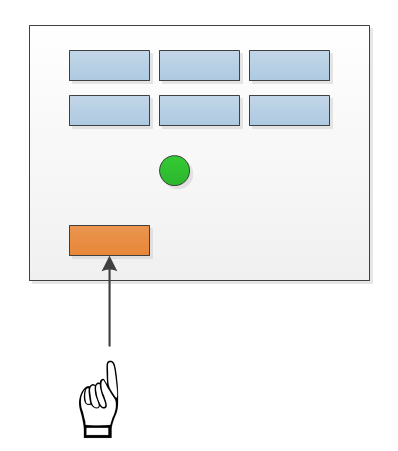
\includegraphics[width=60mm]{Pointer1}}
\subfigure[Right position]{\label{fig:b}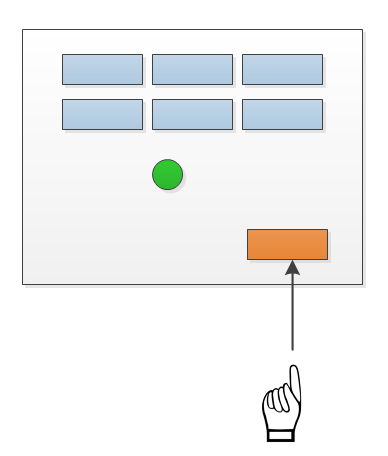
\includegraphics[width=60mm]{Pointer2}}
\caption{Left to right paddle control in breakout using the hand position relative to the screen }
\label{fig:HandPosition}
\end{figure}

\begin{figure}
\centering     %%% not \center
\subfigure[Left Position]{\label{fig:a}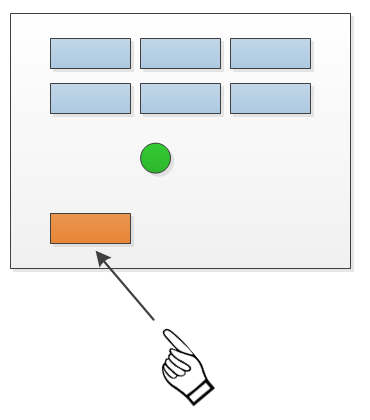
\includegraphics[width=60mm]{PointerIntersect1}}
\subfigure[Right position]{\label{fig:b}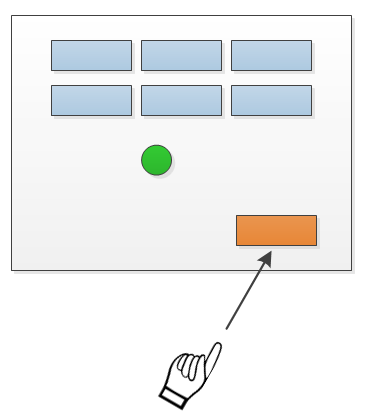
\includegraphics[width=60mm]{PointerIntersect2}}
\caption{Left to right paddle control in Breakout using the pointer intersection with the screen }
\label{fig:PointerIntersect}
\end{figure}

\subsection{Unity}\label{unity_prototype}
One of the main gestures in the requirements used fingers to indicate beginning and ending actions as part of the gesture. Attempting to model these gestures required a 3D environment that could show multiple pointer interactions with game objects which was not possible with Cocos2d. The LeapMotion SDK provided a API with Unity 3D Game Engine which could perform the modeling required to begin recognizing the gestures. It was through this prototype that it was found that the LeapMotion would not be able to detect fingers touching each other\footnote{A later released visualizer in the LeapMotion SDK would show the same result.}. \cite{unity}

\subsection{Quartz 2D}\label{quartz2d_prototype}

The Cocos2d engine is not designed particularly for drawing and rendering textures to images. Apples Quartz 2D and Cocoa libraries are well suited for this task providing a large array of built in functionalities. These libraries were used to create the prototype drawing application using some of the boilerplate code from the earlier Helloworld~\ref{HelloWorld_prototype} and Breakout~\ref{breakout_prototype} prototypes. The boilerplate code formed into a standard interface and coordinate system for working with the LeapMotion. \cite{appleapi}

%%TODO Name for this interface

This prototype worked well in testing in Session 4~\ref{session4} and was generally well received by children although they had one major requirement of adding a cursor in addition to some minor features. The cursor would show where the pointer was on the screen at any given time so they could position it prior to painting. The minor features included selecting brushes, erasing, changing the brush size, changing the brush type and opacity.  

\subsubsection{Challenges}
The cursor was very difficult to implement using the Quartz 2D and Cocoa because the libraries do not natively support layering and drawing simultaneously due to the way the rendering context functions as a single context. Creating independent views and transparent windows did not render correctly when attempting to simultaneously update each view. An alternative might be to put each functionality into separate applications running on different process threads although this was not possible because the LeapMotion can only be accessible from one process at a time. To create a cursor in  HUD layer the application needed to access the LeapMotion, HUD and Drawing objects simultaneously. This was the defining factor in returning to the Cocos2d Game Library because it support independent layering of views. \cite{appleapi}

\subsection{LeapPaint}\label{leappaint_prototype}

The prototype dubbed "LeapPaint" by the children consisted of a combination components from the earlier Helloworld~\ref{HelloWorld_prototype} and Breakout~\ref{breakout_prototype} prototypes managing input on a standard interface and output into different visible for drawing and the HUD. The layers were connected via a GameManager \footnote{GameManager takes the role of the ApplicationDelegate} passing the delegate actions between layers and interfaces. 

This prototype received the best reviews by the children in testing Session 6~\ref{session6} despite lacking some of the features of available in the Quartz 2D~\ref{quartz2d_prototype}. This architecture could be used going forward in adding features.

%despite the tradeoffs between libraries 


\section{User Interface Layout}
The interface layout of controls was based upon a combination of designs made by the children as seen in Figure~\ref{fig:LeapPaintScreenshot} with the canvas to paint on centered and the user interface controls tucked to the sides of the canvas. 


\begin{figure}
\centering     %%% not \center
\subfigure[Mock Up]{\label{fig:a}\includegraphics[width=60mm]{Mockup}}
\subfigure[Screenshot]{\label{fig:b}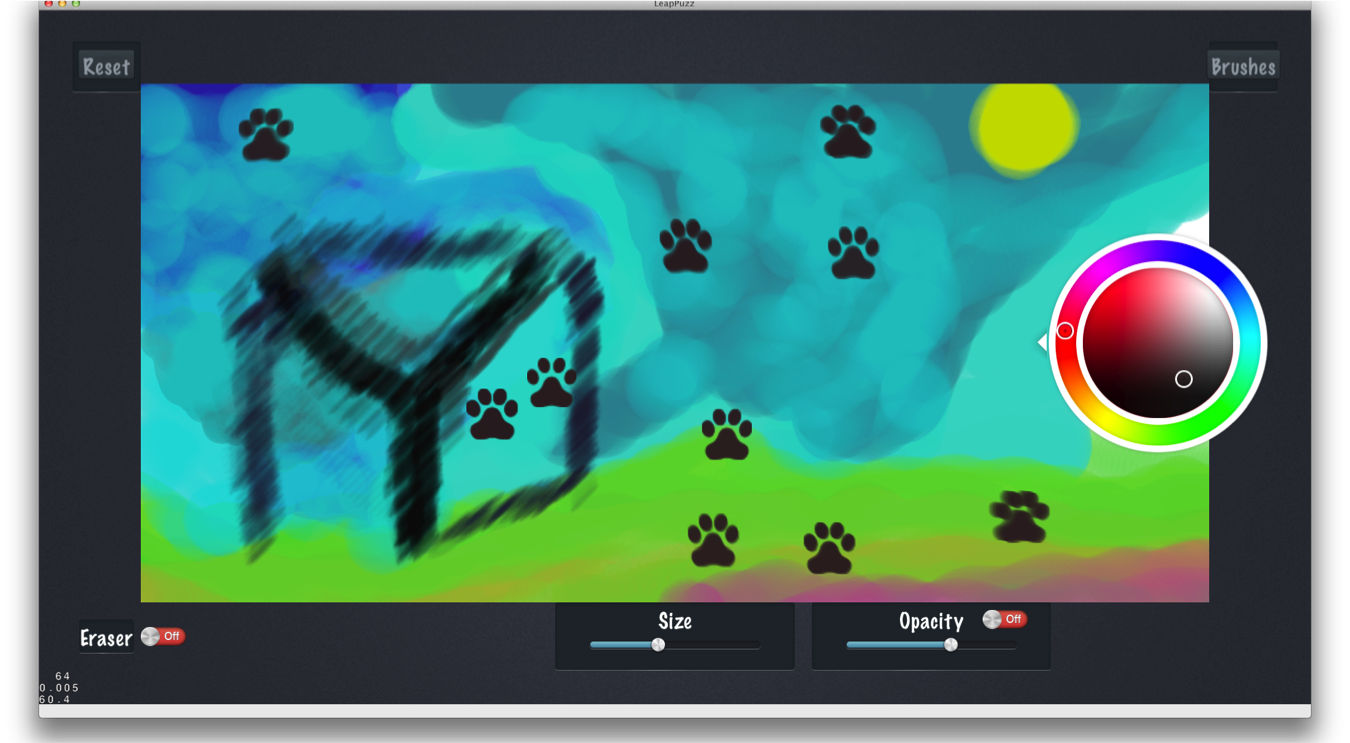
\includegraphics[width=60mm]{LeapPaintScreenshot}}
\caption{Mock up compared to a screen shot of finished application with a drawing. }
\label{fig:LeapPaintScreenshot}
\end{figure}



\subsection{pointer Tracking}
Initially a tracking system was design to use the relative coordinates of a pointer in the LeapMotion coordinate space and translate them to coordinates within the application. Later with the an SDK update the LeapMotion could provide coordinates on the screen where a vector from the pointers tip would intersect. This required some screen calibration to be performed such that the LeapMotion would be able to track points on the screen. 

\subsection{Application Layers}
The application was broken into component layers to manage and modularize different functionalities as seen in Figure~\ref{fig:applicationlayers}. This allowed for some components to become reusable for other applications by providing a common application programming interface (API). 

\begin{figure}
\centering
%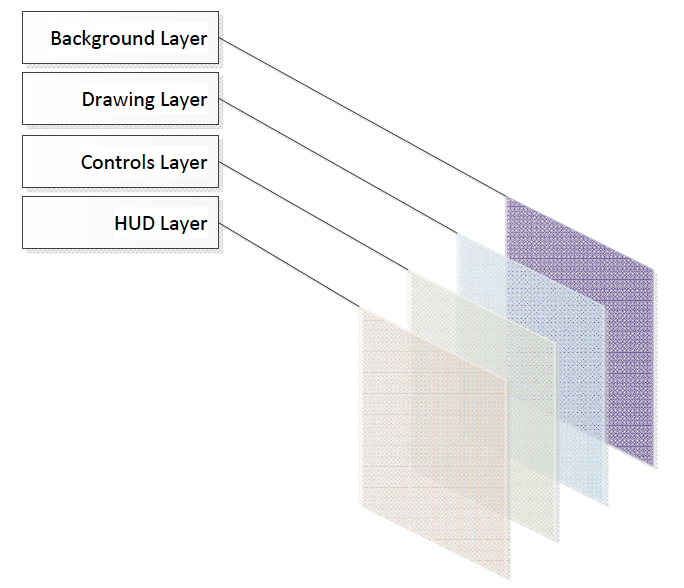
\epsfig{file=applicationlayers, height=0.65\columnwidth, width=\columnwidth}
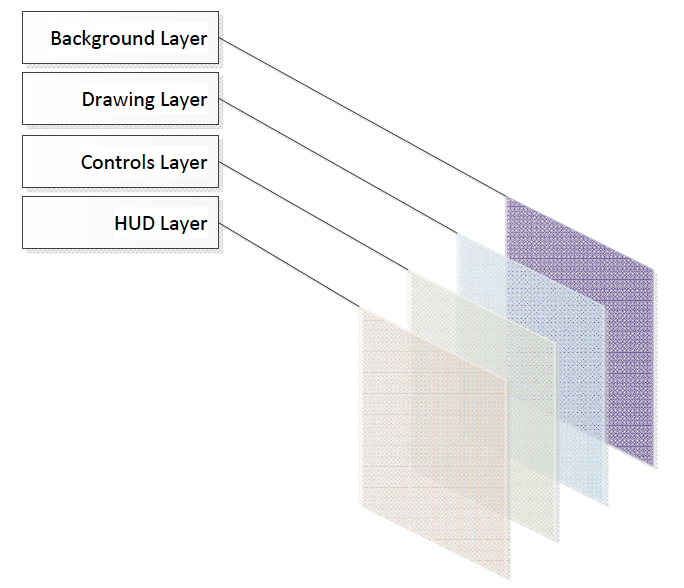
\includegraphics[height=0.65\columnwidth, width=\columnwidth]{applicationlayers}
\caption{The ordered layers of visibility in the application. }
\label{fig:applicationlayers}
\end{figure}

\begin{itemize}
\item Background Layer manages the background images and for the application. This practice is fairly standard and 
\item Drawing Layer is where the image will be edited and render. 
\item Controls Layer provides the user interface controls that for different aspects of the application.
\item HUD Layer displays feedback information for the position of the pointer in relation to the screen and any different actions that might be taking place. 
\end{itemize}

\section{External Libraries}

\begin{itemize}
\item LeapMotion SDK is the provided API for using with the LeapMotion.\cite{leapmotion}
\item Cocos2d is a game engine framework that allows simple animation and control of sprites and layers. \cite{cocos2d}
\item CCControlExtensions are user interface control elements built for the Cocos2d Engine. \cite{cccontrolextension}
\item Graphics Recognition Toolkit was used initially for doing gesture recognition with customized pipeline until a LeapMotion SDK update provided the same functionality. \cite{GRT}

\end{itemize}

\section{Testing}

The project uses unit testing on all the class functions to verify their input and outputs correspond to their intended function. Using the simple methodology of making the test fail and then making the test pass with a variety of inputs and outputs helped modularize class functionality into smaller and more reusable sections. The testing framework OCUnit tests at class and bundle levels to produce full code test coverage. Performing this step on each function refined the design by directly questioning each sub components role and required functionality.\cite{appleapi}

Parts of the project unit testing could not cover were mostly involved at the interface level where the LeapMotion SDK provided data. Environmental factors effect the LeapMotions performance when in a different lighting conditions. The different types and positions of lighting caused erratic effects that often had to be compensated for when noticed. 

\section{Documentation}

Code documentation is done with in-line comments and then automatically generated with Doxygen. This was an essential tool due to the ever changing state of the project during each cycle that the project be able to automatically reflect changes in the design. 

\section{Experimental Features}
Several experimental interface designs were added for the children to test with since there were often more than one design approach to a features in the application. The approached attempted to leverage the 3D space available to the LeapMotion that is not available to the keyboard and mouse. 
\subsection{Drawing Modes}

Two different drawing modes were tested with the children in Session 7~\ref{session7}. The first was a mode where the pointer would begin drawing when crossing a boundary on the Z axis toward the screen. The cursor could then be moved about the screen without interacting with the drawing by pulling the pointer back and then pushing forward when ready to begin drawing. A ring around the cursor icon would indicate weather or not the cursor would begin drawing based on the depth of pointer. The ring would change from red when not in not drawing state to green when beginning to draw. Further development might include a yellow color ring indicator when approaching the threshold to transition states. 

The children did not like using the depth mode option of drawing compared to the spacebar mode bar of drawing  as they had trouble becoming accustom to the threshold in which the application would begin and stop drawing. They did like that they could draw and change colors at the same time by using their free hand with the mouse to create continuous rainbow effects with the brush.  

The second drawing mode was to begin drawing when pressing the space bar on the keyboard and disregarding the depth of the pointer. This proved to be the favorite method of input for the children to indicate their actions. 

\subsection{Depth Opacity}

Another option explored was using the Z axis to control the opacity of the brush. The intent was to provide a pressure sensitive brush which would mimic drawing implements in the real world where pressing harder on a paint brush or marker will draw a darker or thicker line. 

The children did like this feature although and preferred it to manually adjusting the opacity with the mouse. This was Dependant on what they were drawing where it was preferable for background colors but not drawing lines. The feature could be improved with adding some brush stroke effects that vary based on the speed of the pointer when drawing. 

 
% Chapter 1

\chapter{Summary} % Main chapter title

\label{Chapter5} % For referencing the chapter elsewhere, use \ref{Chapter1} 

\lhead{Chapter 5. \emph{Summary}} % This is for the header on each page - perhaps a shortened title

%----------------------------------------------------------------------------------------

\section{General Observations}
The children would first sketch an outline of their drawing and then attempt to color in their outlines. This proved difficult in the case of the LeapMotion. Drawing the lines proved fairly easy for the children while shading in sections appeared more difficult. I found the opposite to be true of my own experience as the lines were harder to draw than shading in the areas.

\section{Similar Applications}

Comparison to industry competitors Corel's Painter Freestyle which will have many of the same features. In terms of interface design they chose a similar layout of control mechanisms. We haven't be able to to see this all quiet yet since it has not been released to perform a full comparison although from the initial details given on their website seems to lead that their application could be similar to ours in many respects. \cite{corelfreestyle}

\subsection{Google Earth}
Examples of dedication are shown in some example applications where the LeapMotion has a specific purpose. Google Earth uses it for navigation only allowing the user to pan, rotate and elevated the camera in relation to the earth. Interpreting the hand motions as the path of airplane as the control mechanism with yaw, pitch, roll, bank and elevation. 

The way of controlling the Google Earth is similar to the idea of controlling the Temple Run game brainstormed in from Session 1~\ref{session1}. This connection was not apparent when first considering the idea for controlling the game. 

\section{Conclusions}
The LeapMotion is a great device for capturing the motions and positions of the hand in real time but is tough to consider as replacement for the keyboard and mouse. It is foreseeable that the main application for the LeapMotion will not be as a general use device but for specific applications which enable expressive movement. Games, drawing and music applications are good examples of where the LeapMotion can focus on specialized actions. Integration into general purpose applications will be difficult due to existing designs and interface paradigms. 




%Integration with other devices such as mounting on a keyboard or embedding into a laptop or monitor will 


%%In the initial phases terminology cocolily synomous with the mouse was avoided. 


 

%% Chapter 1

\chapter{Not named Chapter} % Main chapter title

\label{Chapter5} % For referencing the chapter elsewhere, use \ref{Chapter1} 

\lhead{Chapter 5. \emph{Not named chapter}} % This is for the header on each page - perhaps a shortened title

%----------------------------------------------------------------------------------------

\subsection{Observations}
The children would first sketch an outline of their drawing and then attempt to color in their outlines. This proved difficult in the case of the LeapMotion. Drawing the lines proved fairly easy for the children while shading in sections appeared more difficult. I found the opposite to be true of my own experience as the lines were harder to draw than shading in the areas.

The LeapMotion is so sensitive that it often has to be averaged out to reduce the noise in which is received from raw data. 

\section{Similar Applications}

Comparison to industry competitors Corel's Painter Freestyle which will have many of the same features. In terms of interface design they chose a similar layout of control mechanisms. We haven't be able to to see this all quiet yet since it has not been released to perform a full comparison although from the initial details given on their website it seems that their application could be similar to ours in many respects. \cite{corel}

\section{Google Earth}
Examples of dedication are shown in some example applications where the LeapMotion has a specific purpose. Google Earth uses it for navigation only allowing the user to pan, rotate and elevated the camera in relation to the earth. Interpreting the hand motions as the path of airplane as the control mechanism with yaw, pitch, roll, bank and elevation. 

\section{Summary}
With work extending into different areas of how the leapmotion could be used to control
<FIX>
\section{Future Research}
Some Future Research go here <FIX>

\section{Acknowledgments}
We would like to thank Montclair State University and our child design partners forming KidsTeam.

\section{Afterward}
Collaborative design with only one LeapMotion proved to be difficult as only one child could use the LeapMotion at a time. This was disappointing in some respects. <Fix>


 
%\input{./Chapters/Chapter7} 

%----------------------------------------------------------------------------------------
%	THESIS CONTENT - APPENDICES
%----------------------------------------------------------------------------------------

\addtocontents{toc}{\vspace{2em}} % Add a gap in the Contents, for aesthetics

\appendix % Cue to tell LaTeX that the following 'chapters' are Appendices

% Include the appendices of the thesis as separate files from the Appendices folder
% Uncomment the lines as you write the Appendices

% Appendix A

\chapter{Documentation} % Main appendix title

\label{AppendixA} % For referencing this appendix elsewhere, use \ref{AppendixA}

\lhead{Appendix A. \emph{Documentation}} % This is for the header on each page - perhaps a shortened title

%Write your Appendix content here.

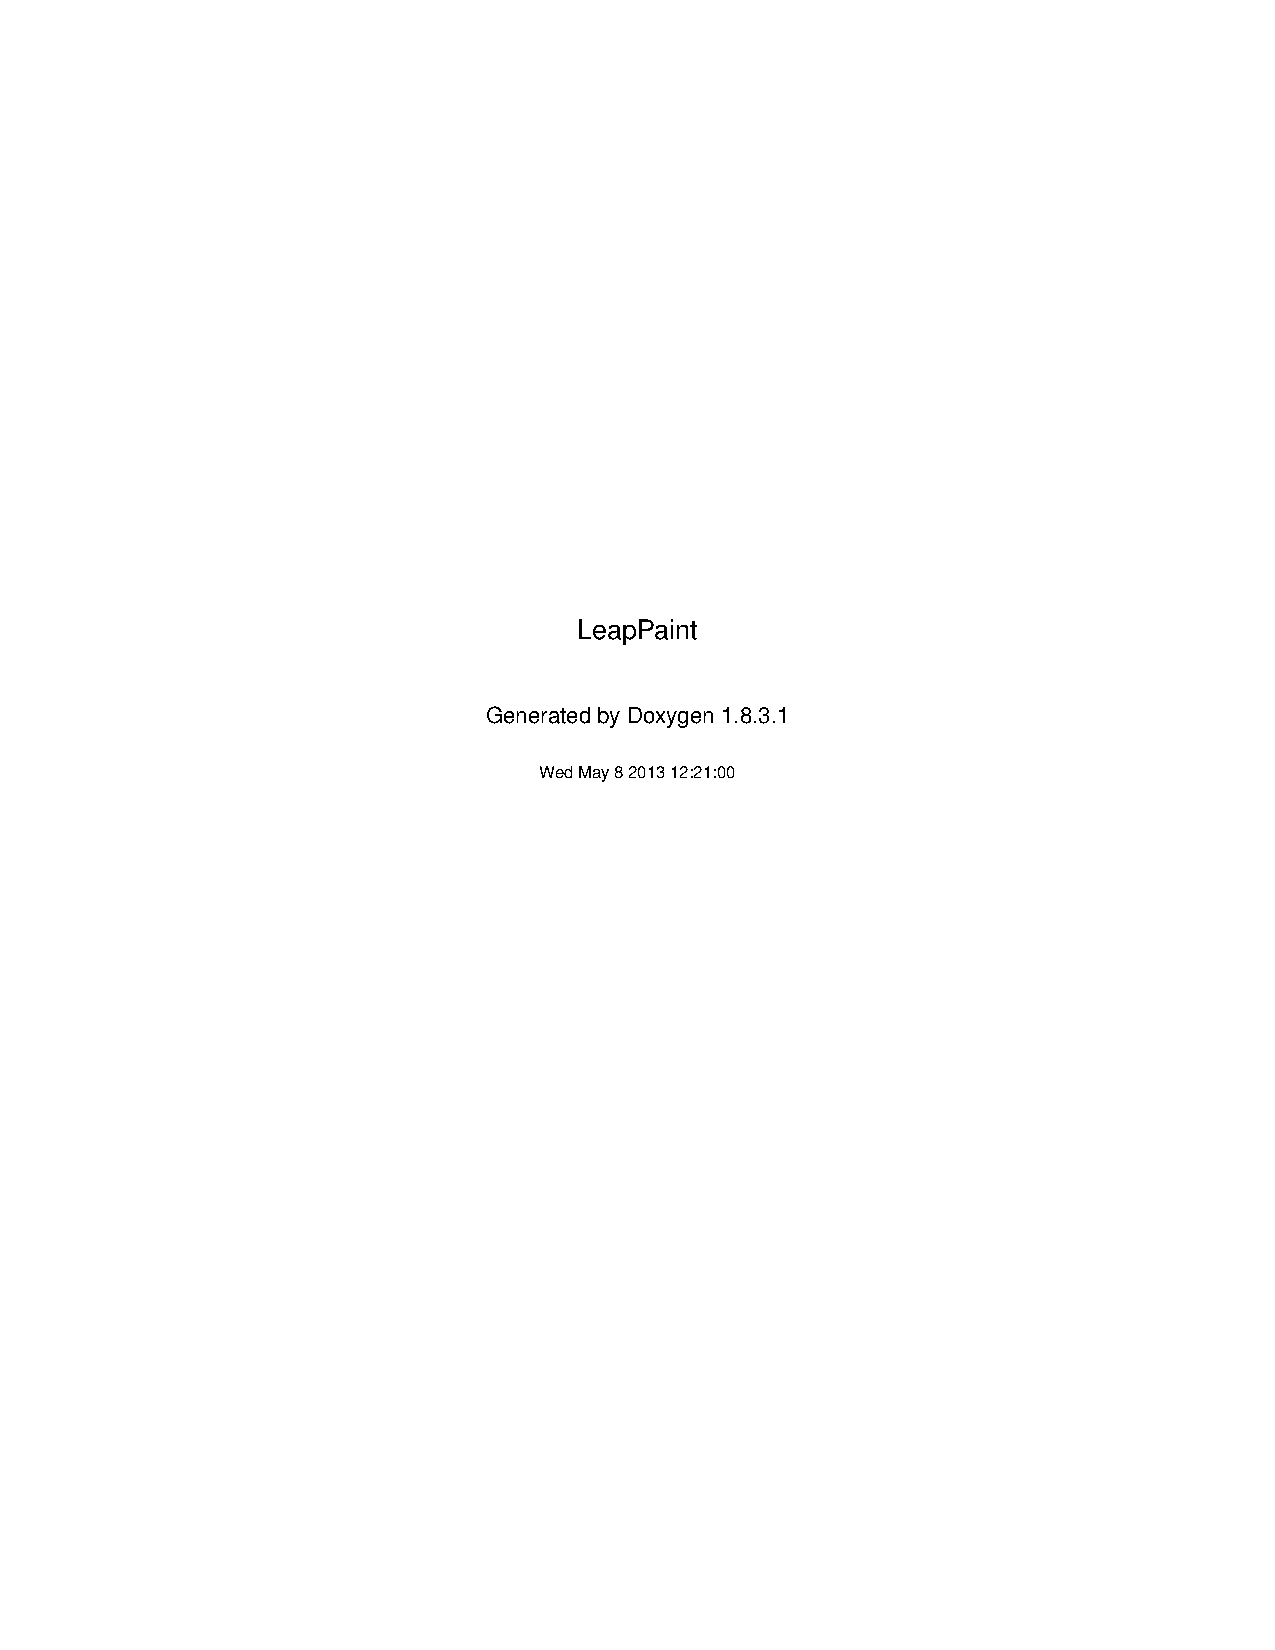
\includepdf[pages=2-last,
	    pagecommand={\thispagestyle{empty}},
            %width=\textwidth,
            %height=\textheight, 
	    noautoscale,   
	    fitpaper=true,
            %offset=0pt 0pt,     %letter, oneside    => misaligned by .x pt
            offset=70pt 0pt,  %letter, twoside    => misaligned by .x pt
            %offset=0pt 0pt,    %a4paper, oneside   => misaligned by 1.x pt
            %offset=-25pt 0pt,  %a4paper, twoside   => misaligned by 1.x pt
            ]{/Users/cj/Desktop/MastersProject/LeapPaint/docs/latex/refman.pdf}


%include each project

% Appendix B

\chapter{Specification} % Main appendix title

\label{AppendixB} % For referencing this appendix elsewhere, use \ref{AppendixA}

\lhead{Appendix B. \emph{Specification}} % This is for the header on each page - perhaps a shortened title

%Write your Appendix content here.

/import{specification.tex}
%% Appendix C

\chapter{BreakOut} % Main appendix title

\label{AppendixB} % For referencing this appendix elsewhere, use \ref{AppendixA}

\lhead{Appendix C. \emph{BreakOut}} % This is for the header on each page - perhaps a shortened title

%Write your Appendix content here.
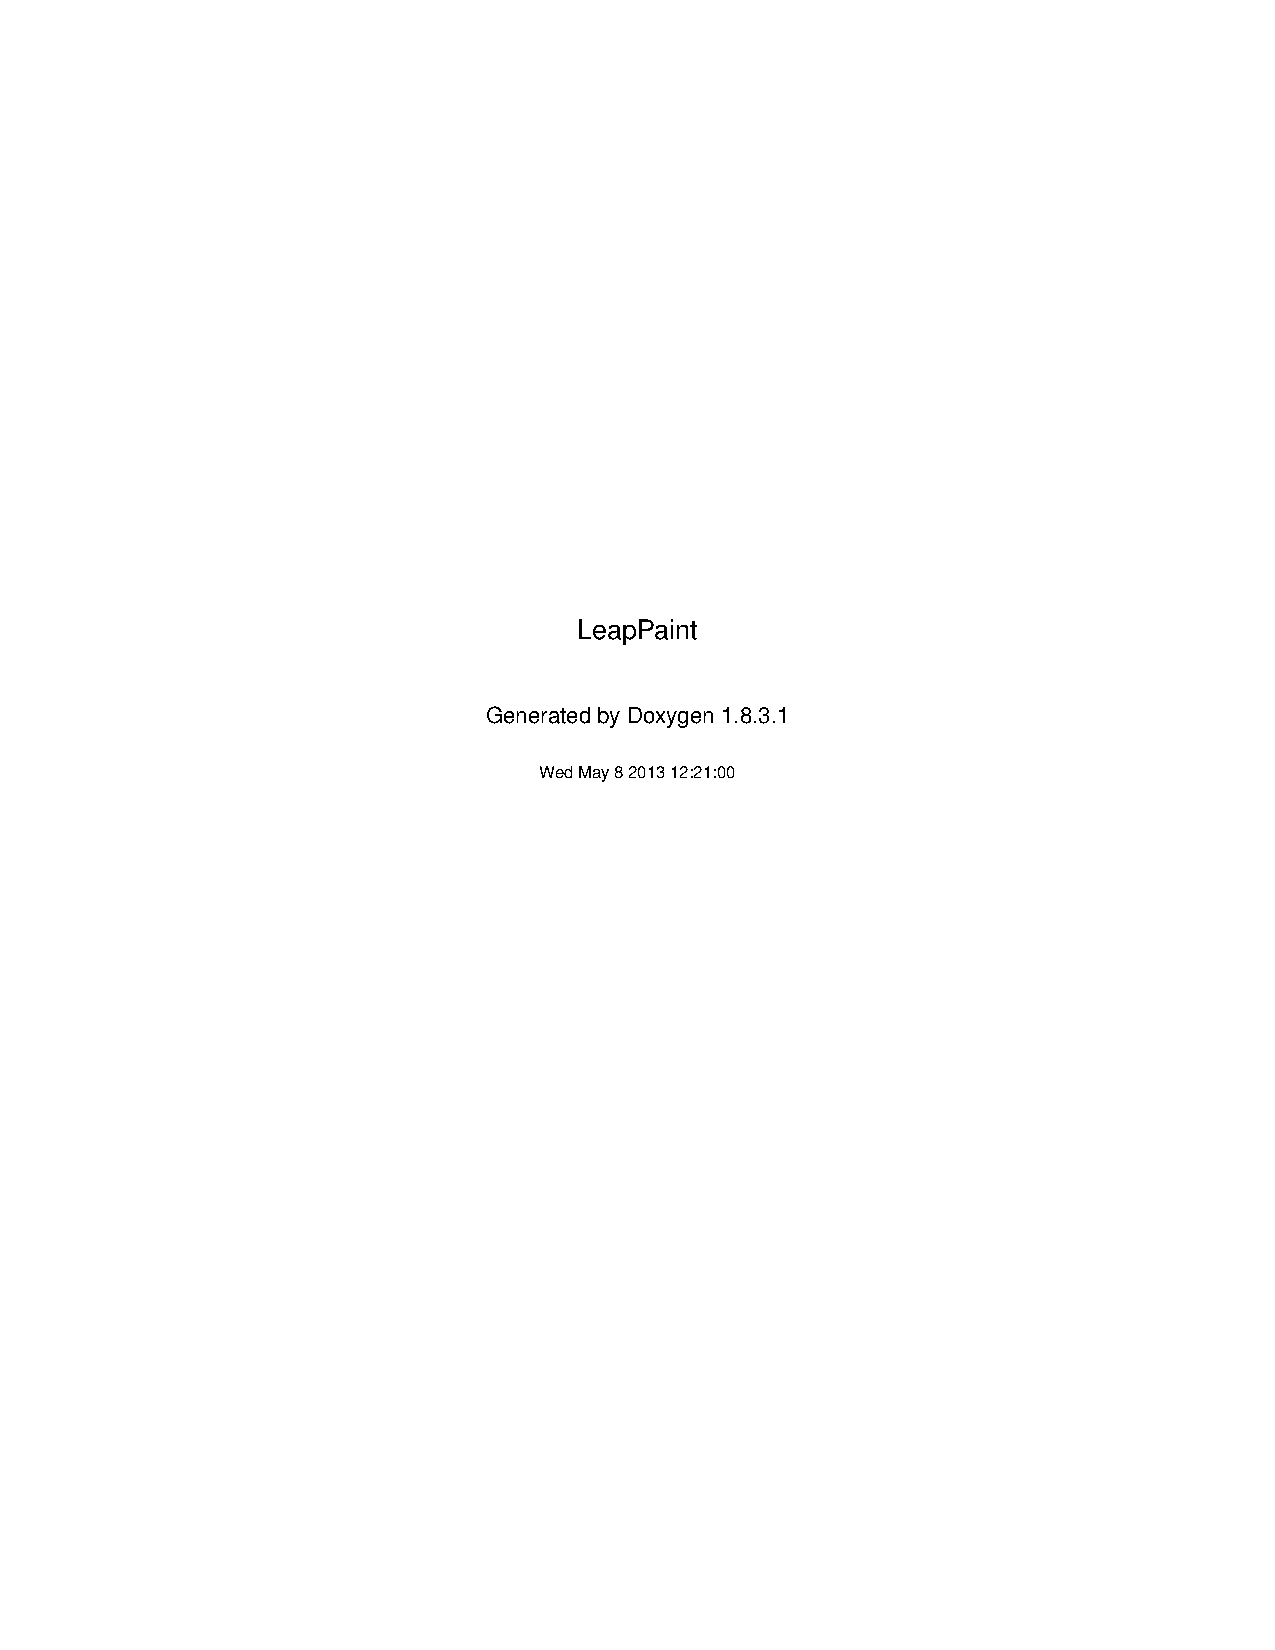
\includepdf[pages=2-last,
	    pagecommand={\thispagestyle{empty}},
            width=\textwidth+ \marginparwidth +\marginparwidth,
            height=\textheight , 
	    noautoscale,   
	    fitpaper=true,
            %offset=0pt 0pt,     %letter, oneside    => misaligned by .x pt
            offset=70pt -70pt,  %letter, twoside    => misaligned by .x pt
            %offset=0pt 0pt,    %a4paper, oneside   => misaligned by 1.x pt
            %offset=-25pt 0pt,  %a4paper, twoside   => misaligned by 1.x pt
            ]{/Users/cj/Desktop/MastersProject/BreakOut/docs/latex/refman.pdf}

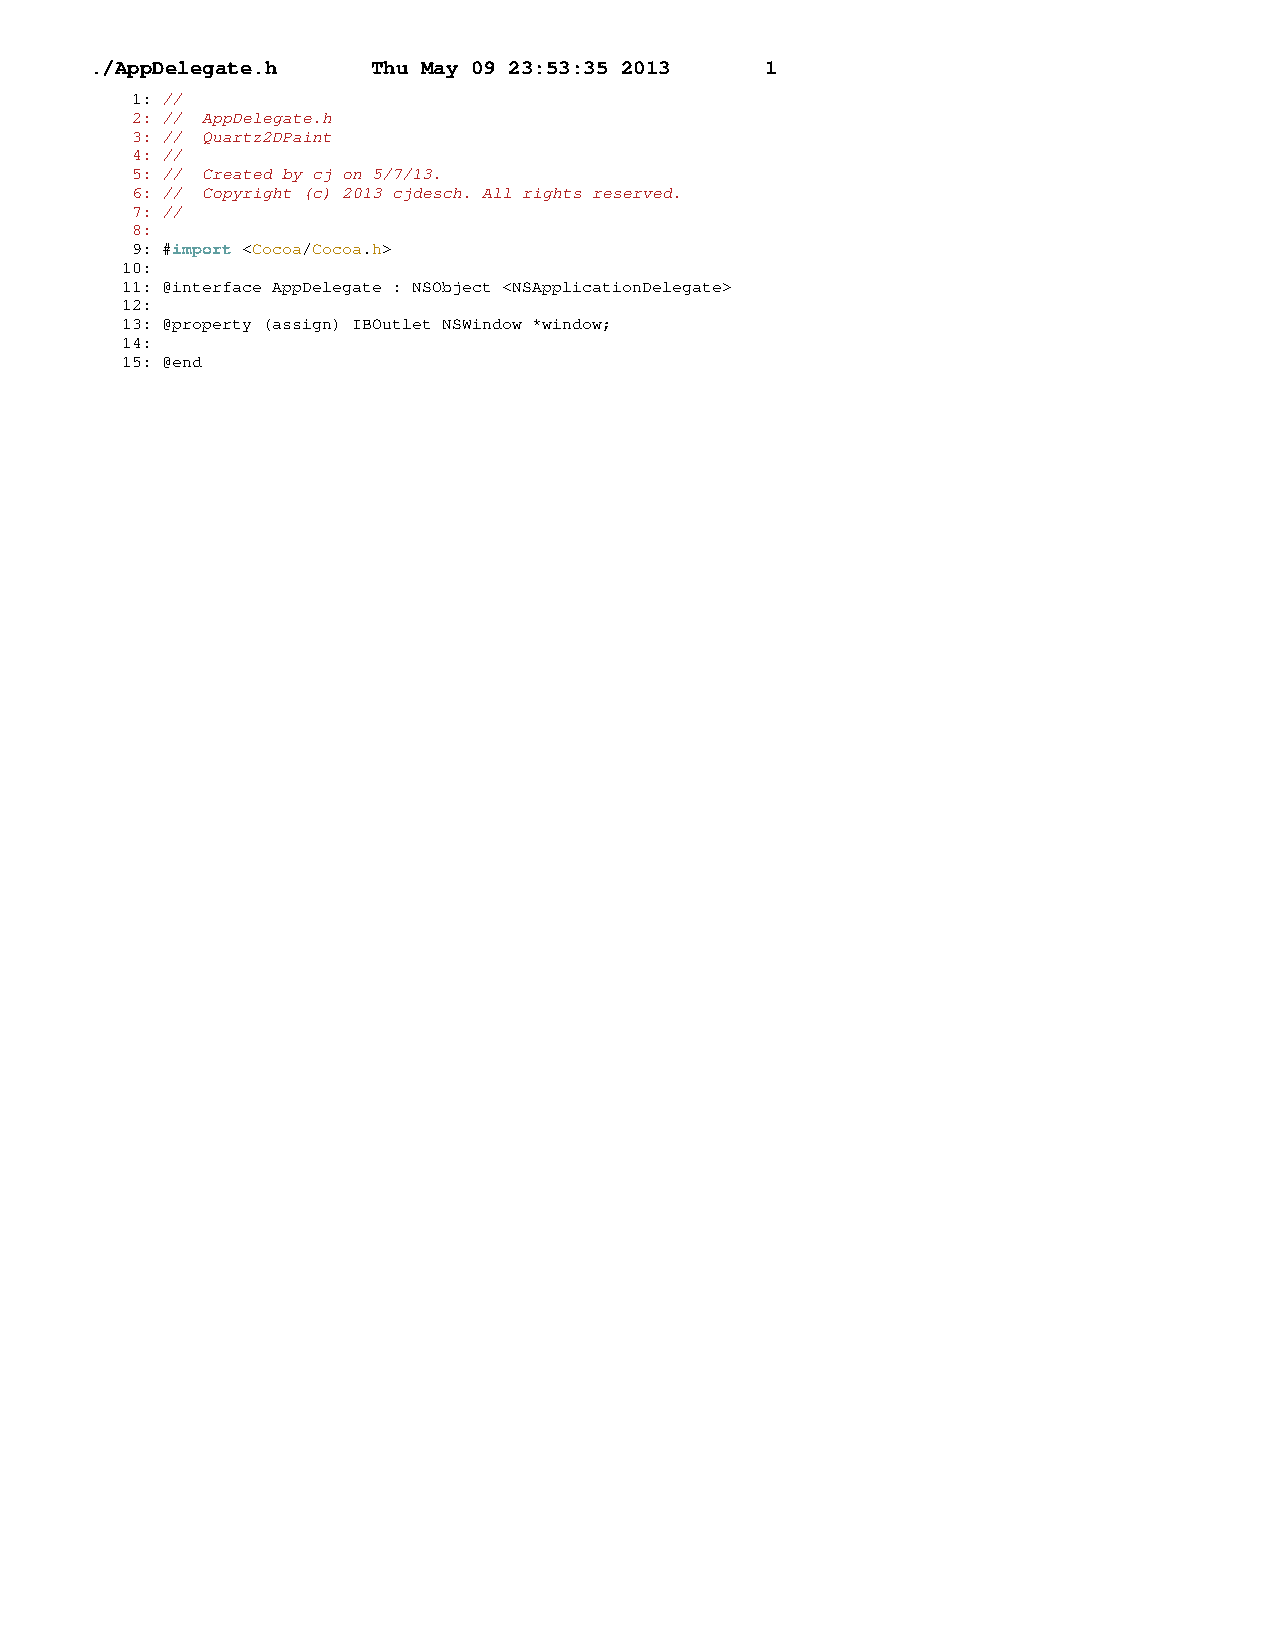
\includepdf[pages=-,
	    pagecommand={\thispagestyle{empty}},
            width=\textwidth,
            height=\textheight, 
	    noautoscale,   
	    fitpaper=true,
            %offset=0pt 0pt,     %letter, oneside    => misaligned by .x pt
           % offset=70pt 0pt,  %letter, twoside    => misaligned by .x pt
            %offset=0pt 0pt,    %a4paper, oneside   => misaligned by 1.x pt
            %offset=-25pt 0pt,  %a4paper, twoside   => misaligned by 1.x pt
            ]{/Users/cj/Desktop/MastersProject/BreakOut/BreakOut/code.pdf}

\addtocontents{toc}{\vspace{2em}} % Add a gap in the Contents, for aesthetics

\backmatter

%----------------------------------------------------------------------------------------
%	BIBLIOGRAPHY
%----------------------------------------------------------------------------------------

\label{Bibliography}

\lhead{\emph{Bibliography}} % Change the page header to say "Bibliography"

\bibliographystyle{unsrtnat} % Use the "unsrtnat" BibTeX style for formatting the Bibliography

\bibliography{Bibliography} % The references (bibliography) information are stored in the file named "Bibliography.bib"

\end{document}  